% -------------- VR postFit 2J ---------
\begin{figure}[h]
  \centering
    \subfigure[]{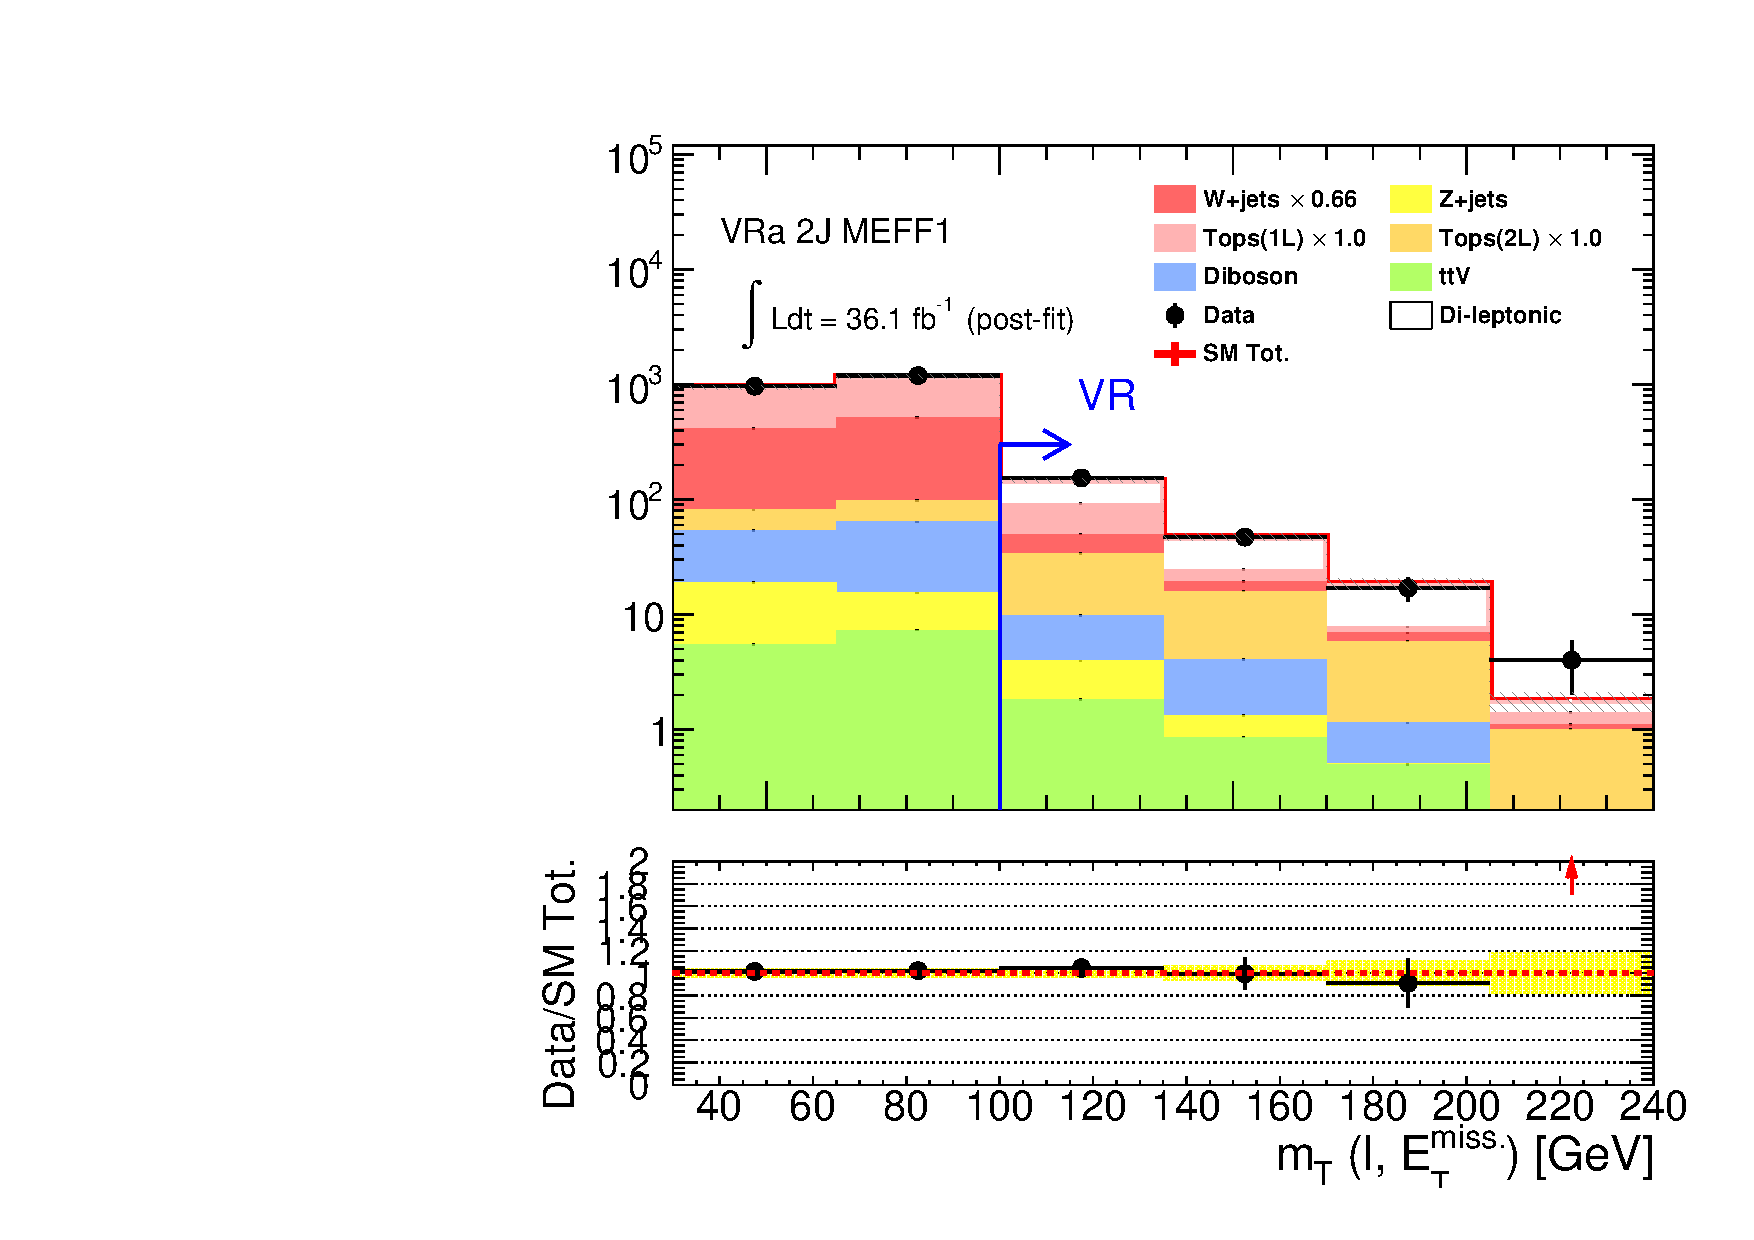
\includegraphics[width=0.41\textwidth]{figures/BGestimation/SRVRpostFit/mt__VRa2JMEFF1_no_mt_postFit_2SFconfig_noYields_objRep.pdf}}
    \subfigure[]{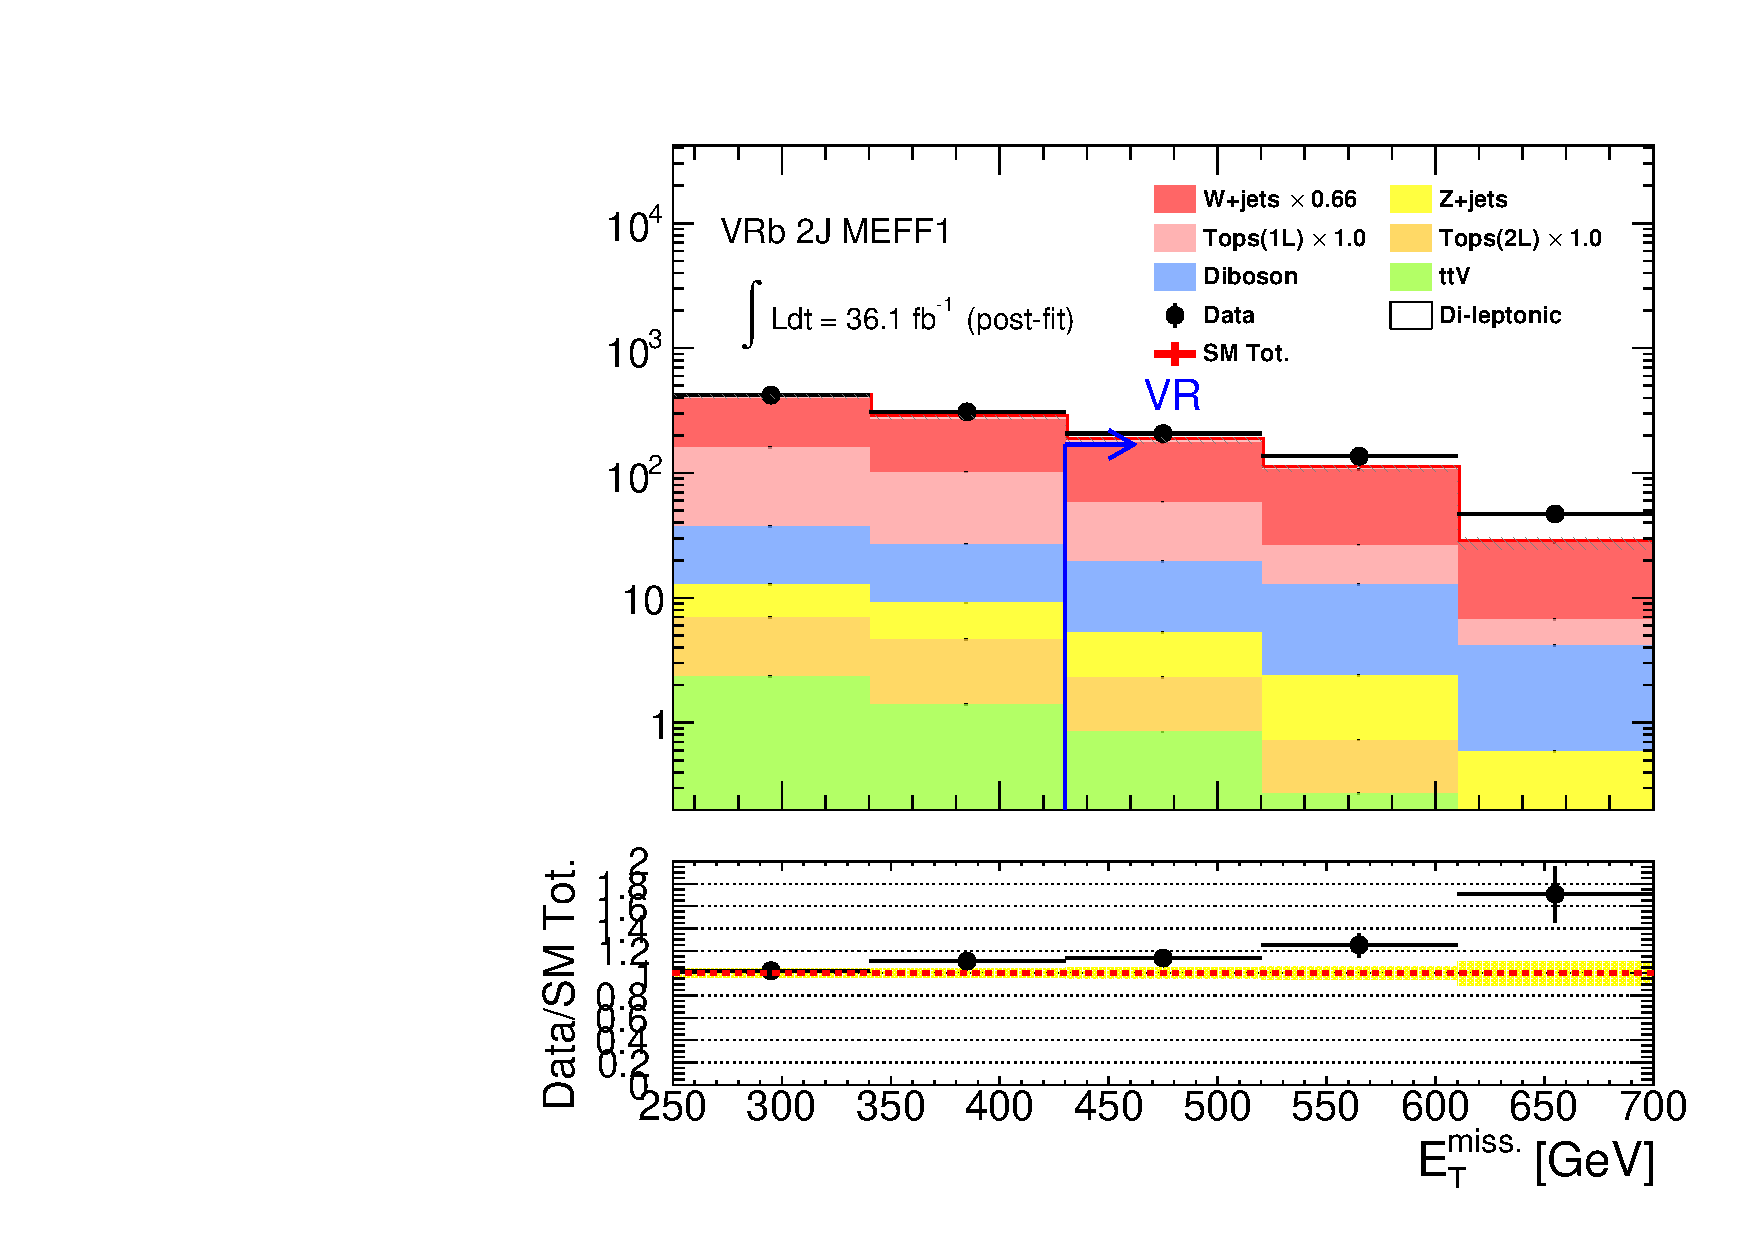
\includegraphics[width=0.41\textwidth]{figures/BGestimation/SRVRpostFit/met__VRb2JMEFF1_no_met_postFit_2SFconfig_noYields_objRep.pdf}}
    \subfigure[]{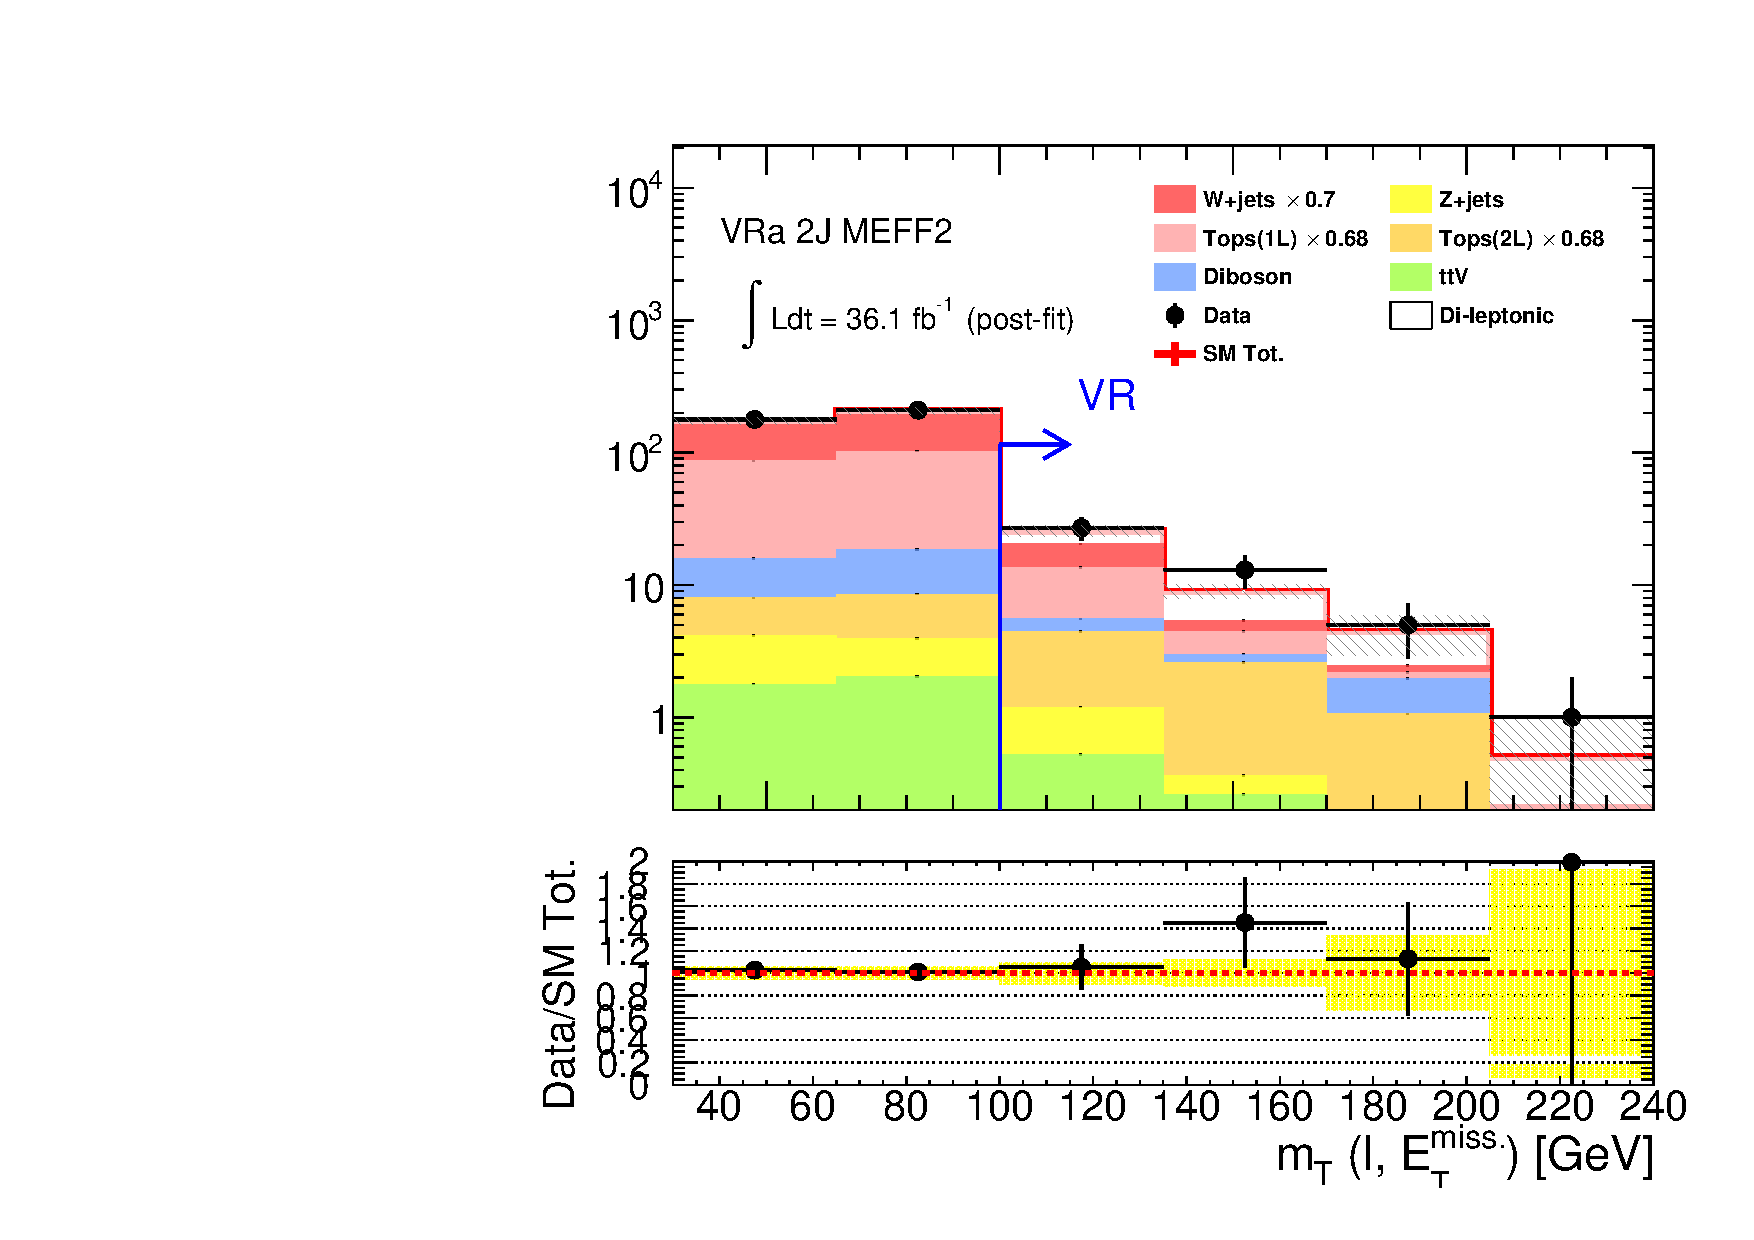
\includegraphics[width=0.41\textwidth]{figures/BGestimation/SRVRpostFit/mt__VRa2JMEFF2_no_mt_postFit_2SFconfig_noYields_objRep.pdf}}
    \subfigure[]{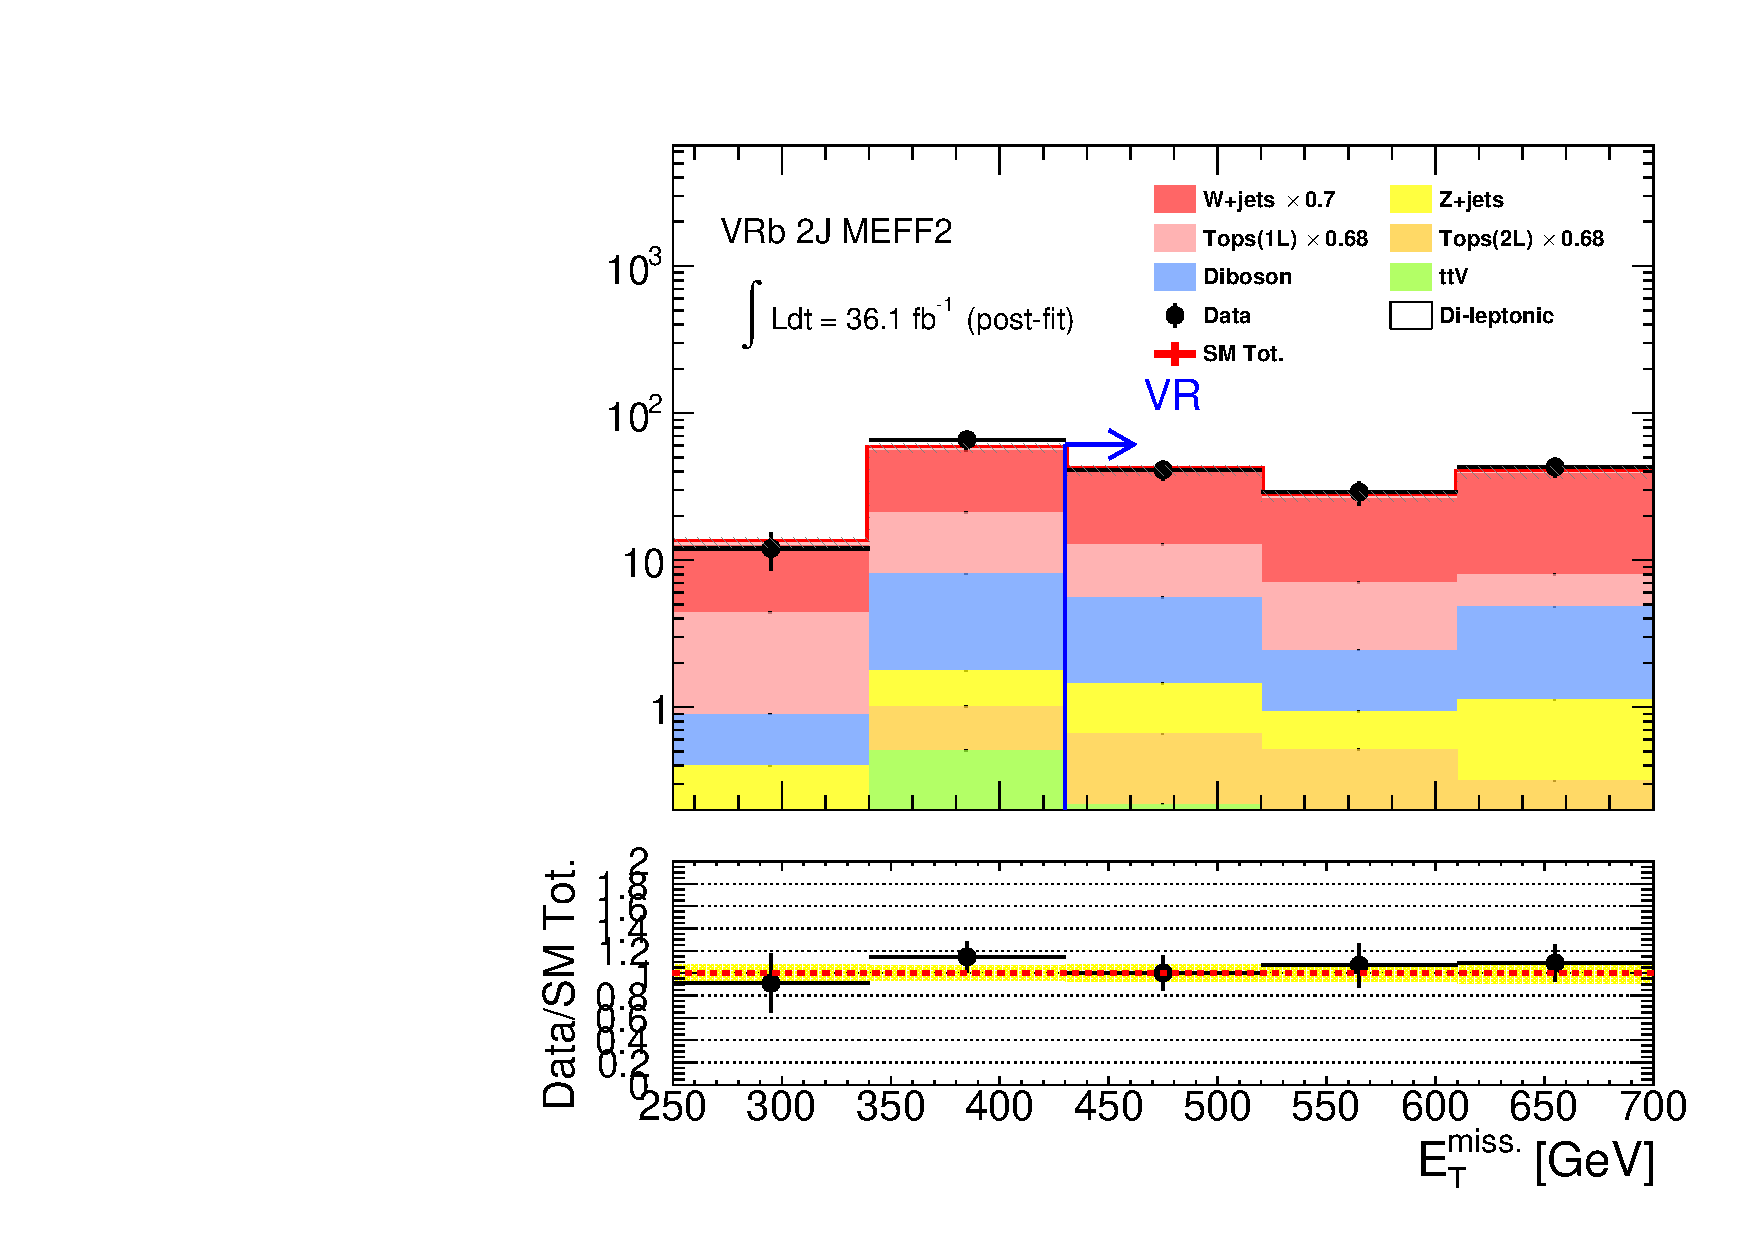
\includegraphics[width=0.41\textwidth]{figures/BGestimation/SRVRpostFit/met__VRb2JMEFF2_no_met_postFit_2SFconfig_noYields_objRep.pdf}}
    \subfigure[]{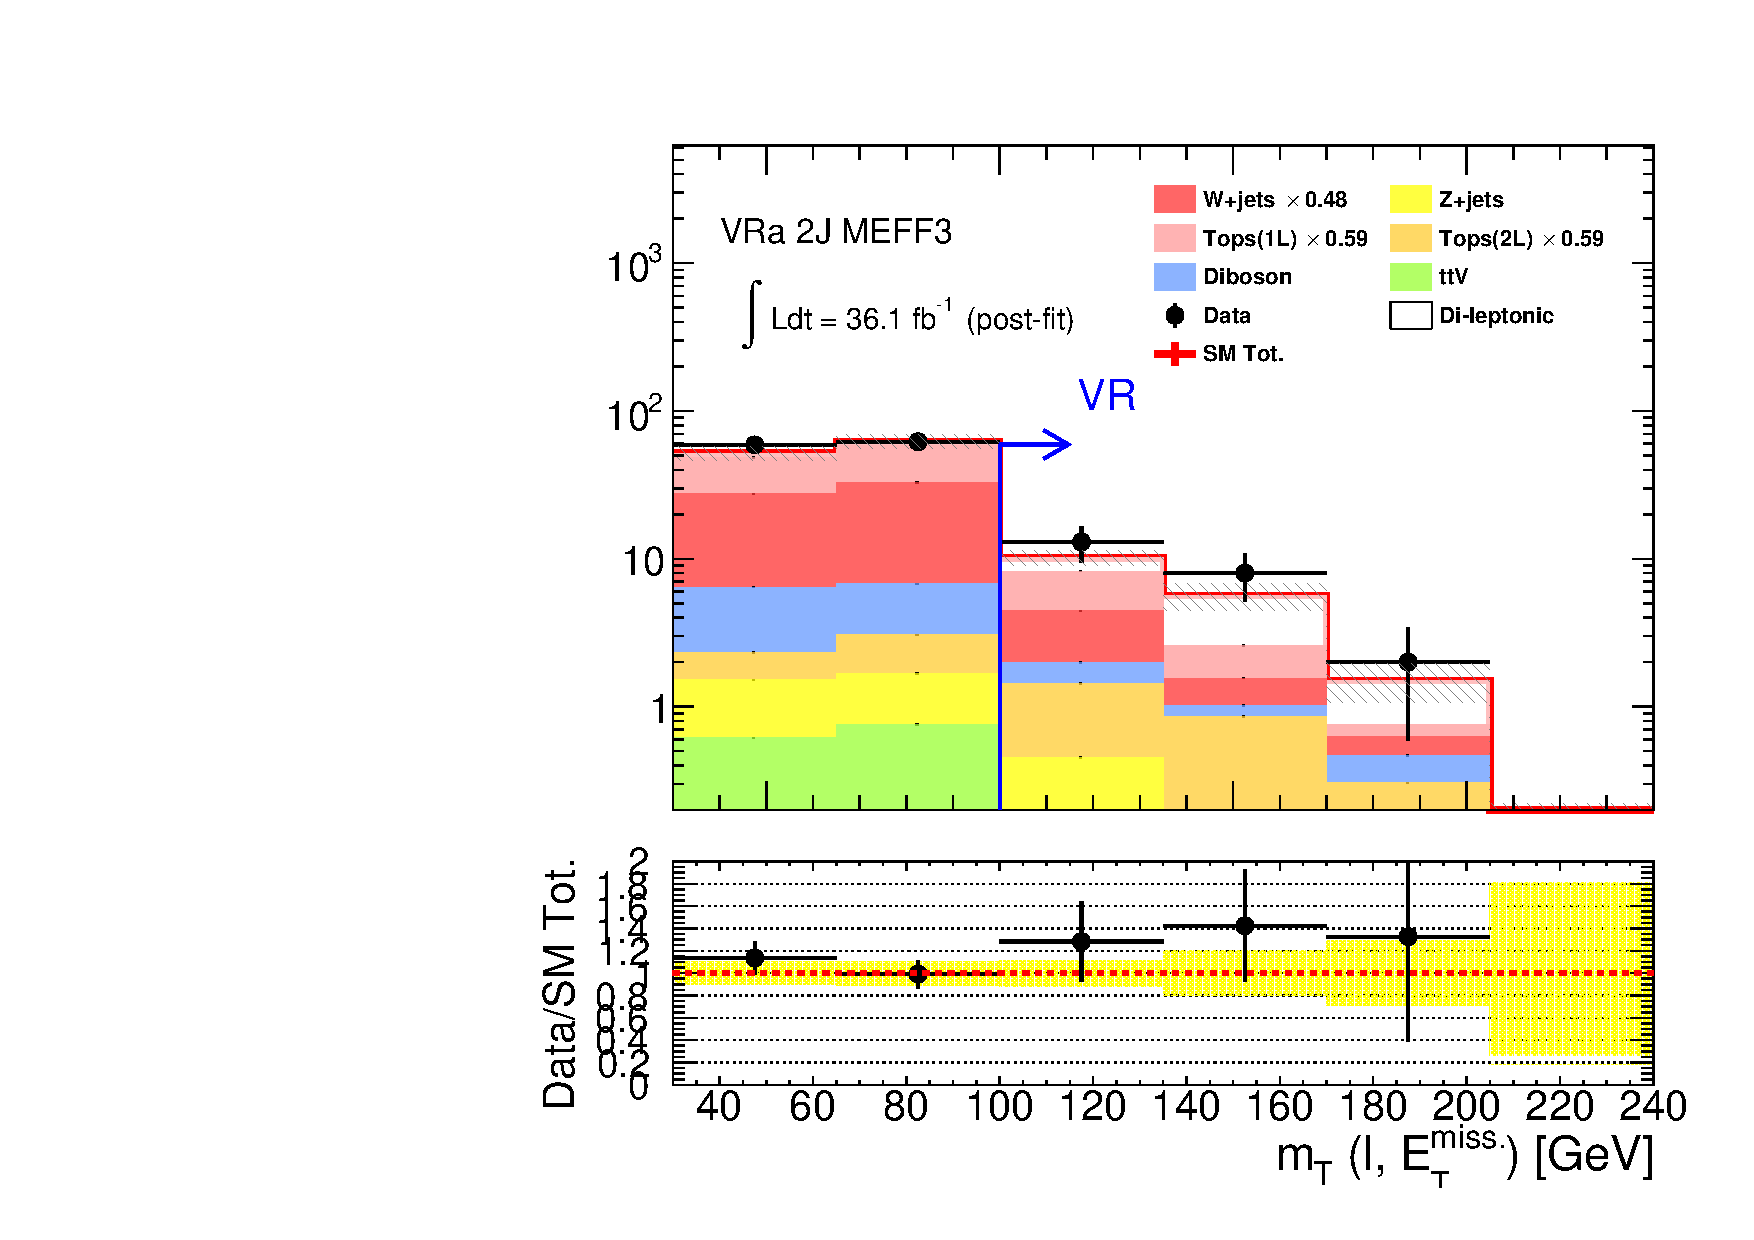
\includegraphics[width=0.41\textwidth]{figures/BGestimation/SRVRpostFit/mt__VRa2JMEFF3_no_mt_postFit_2SFconfig_noYields_objRep.pdf}}
    \subfigure[]{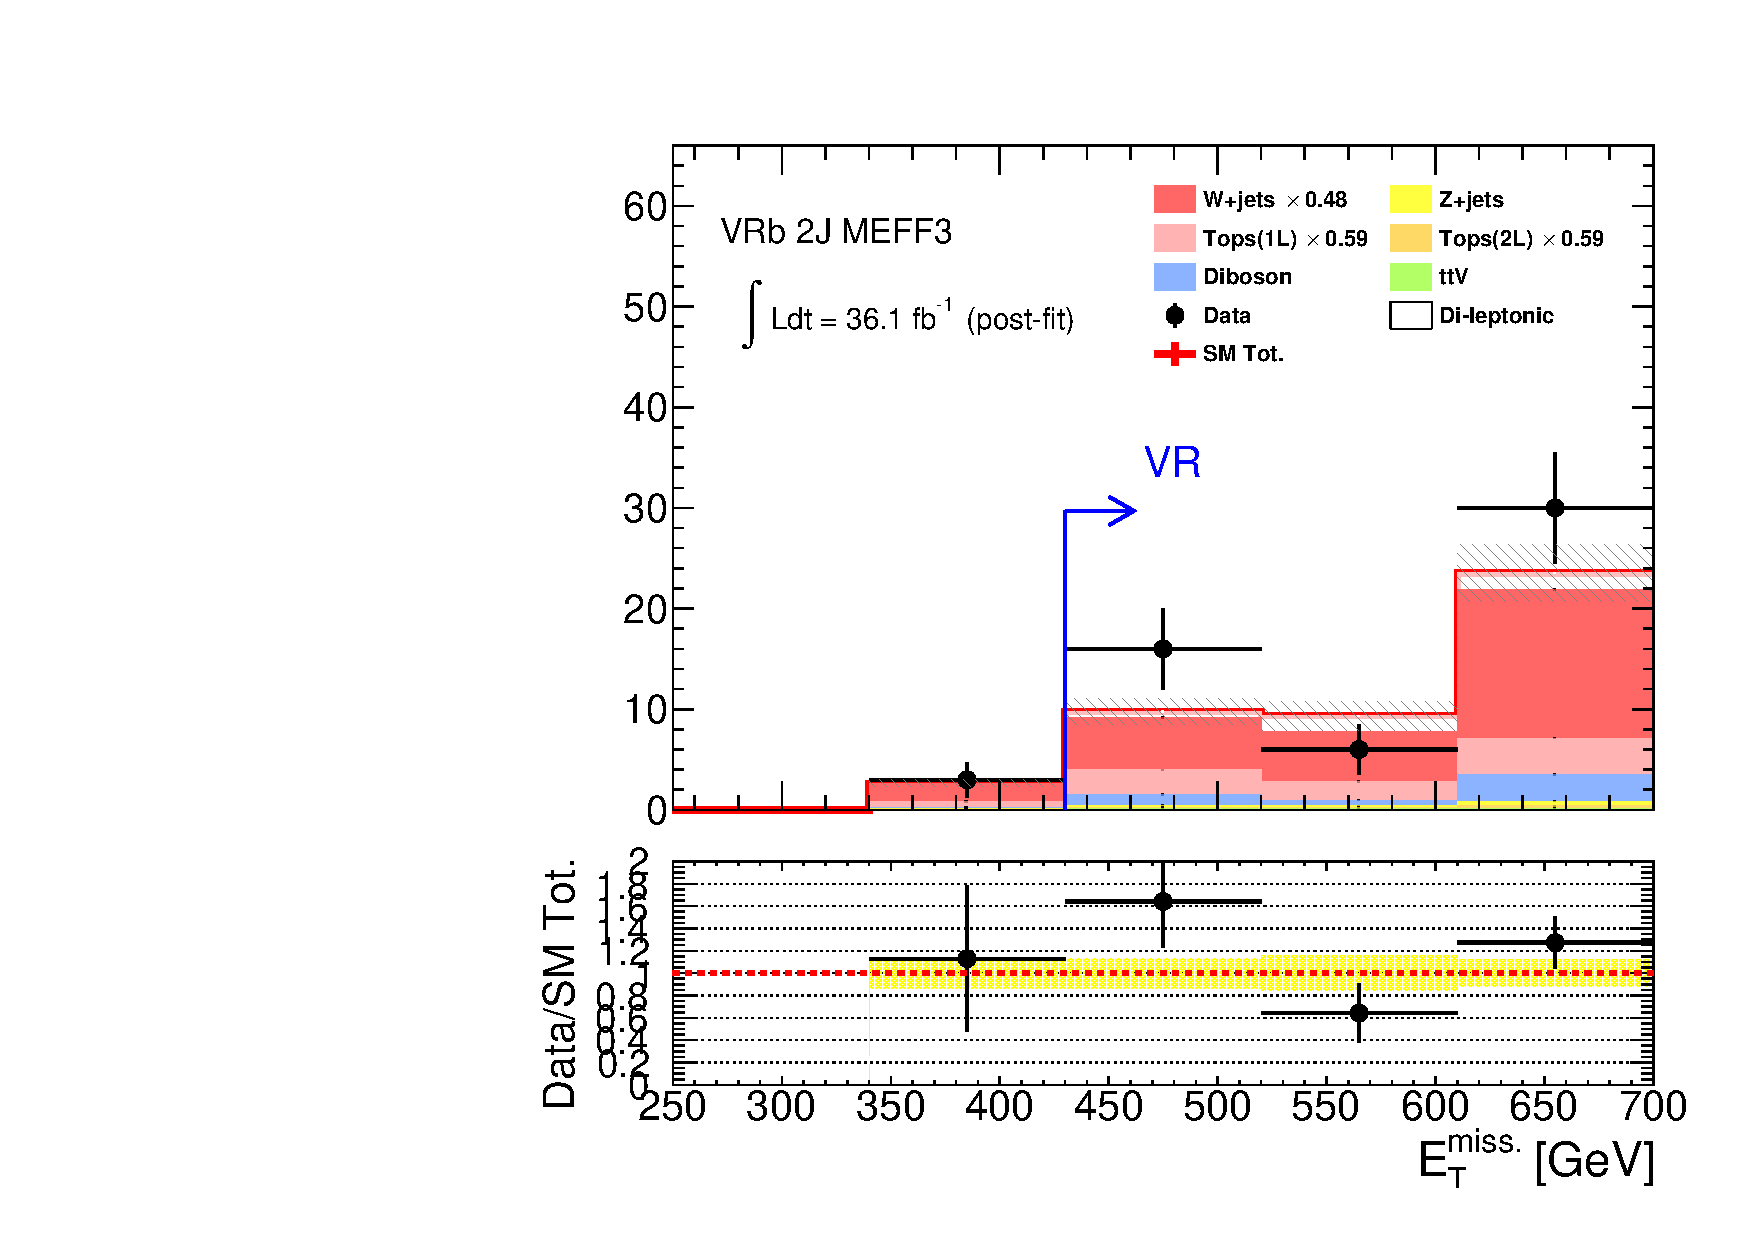
\includegraphics[width=0.41\textwidth]{figures/BGestimation/SRVRpostFit/met__VRb2JMEFF3_no_met_postFit_2SFconfig_noYields_objRep.pdf}}
   \caption{
     Post-fit distruibution of (left) $\mt$ in VRa, and (right) $\met$ in VRb.
     (a,b) VR 2J-$\meffIncFirst$.
     (c,d) VR 2J-$\meffIncSecond$.
     (e,f) VR 2J-$\meffIncThird$. 
     The yellow band in the bottom panel represents statistical error. The overflow is included in the highest bin.  
     \label{fig::BGestimation::SRVRpostFit::VR2J}
   }
\end{figure}

\clearpage
% -------------- 6J ---------
\begin{figure}[h]
  \centering
    \subfigure[]{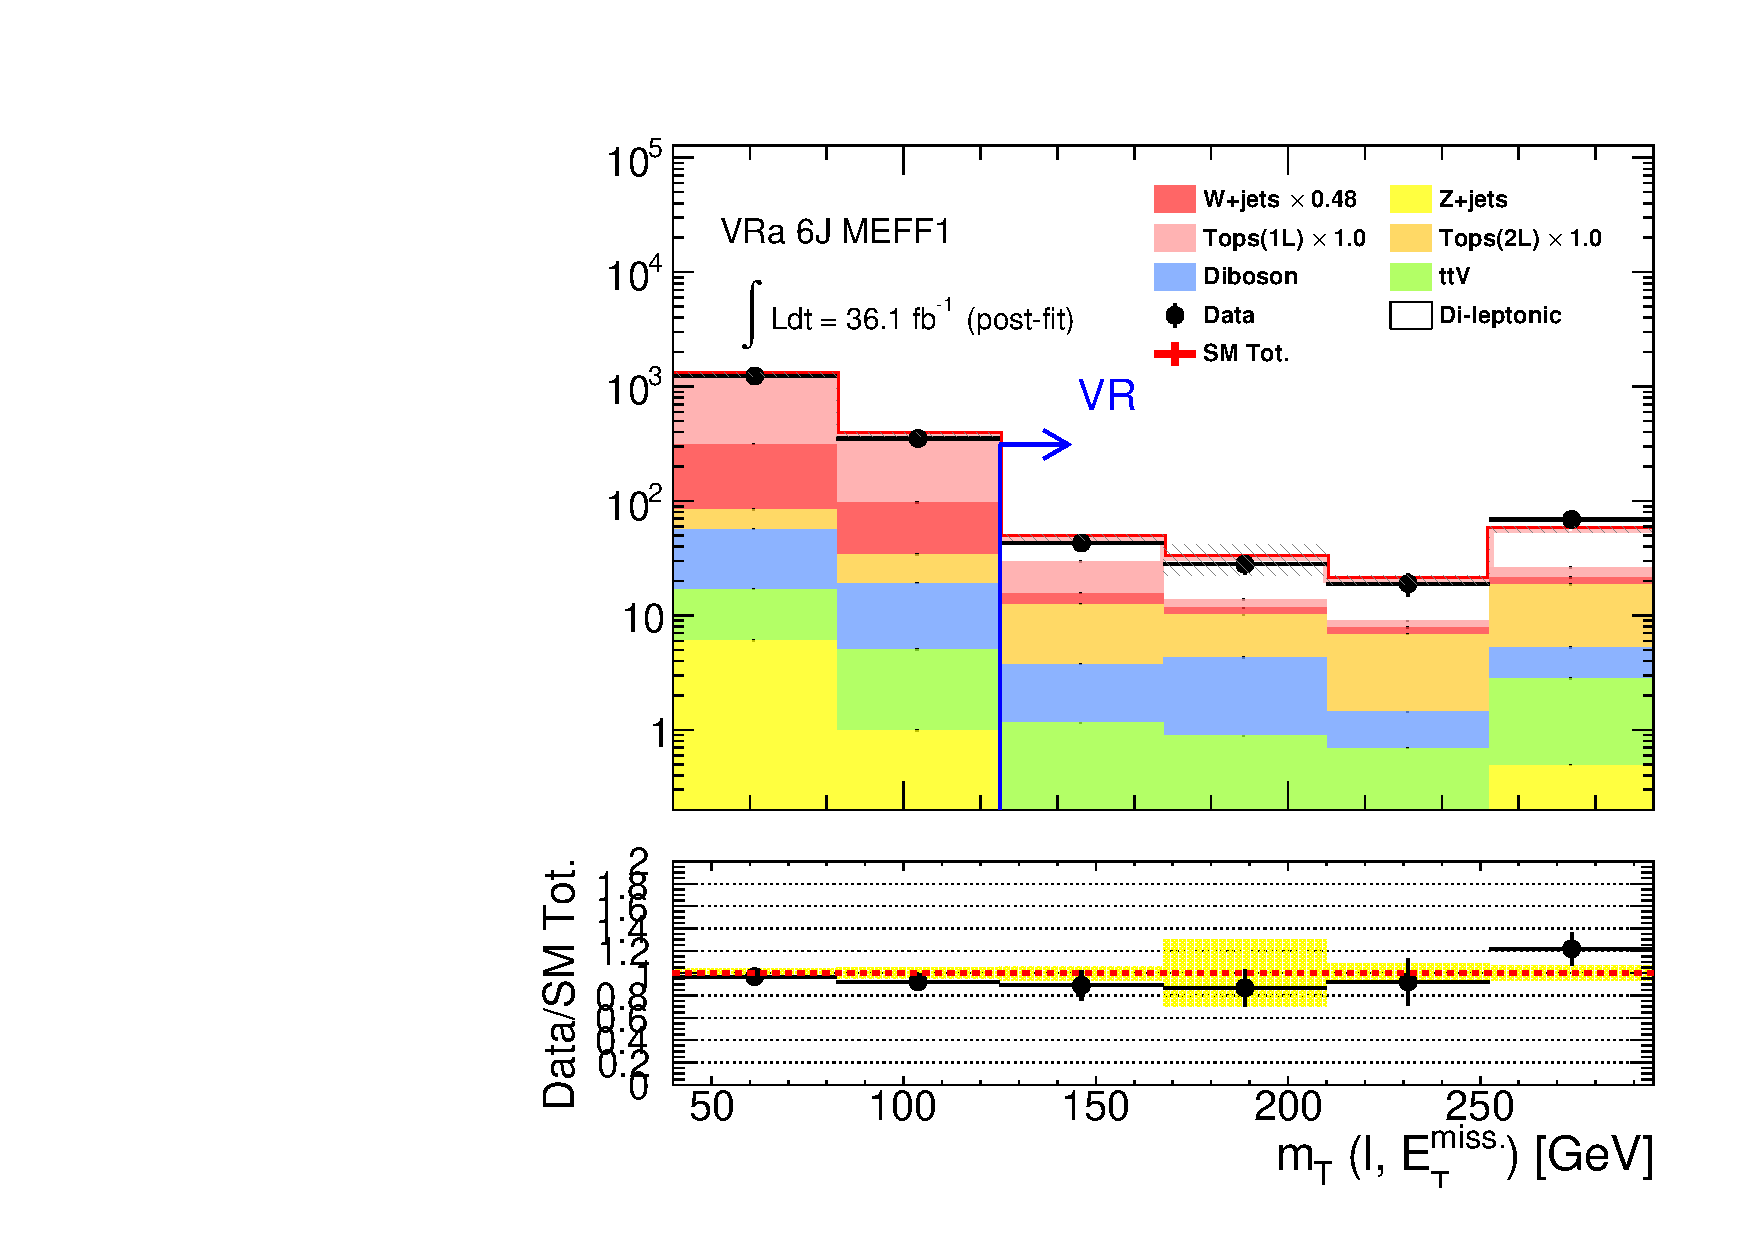
\includegraphics[width=0.41\textwidth]{figures/BGestimation/SRVRpostFit/mt__VRa6JMEFF1_no_mt_postFit_2SFconfig_noYields_objRep.pdf}}
    \subfigure[]{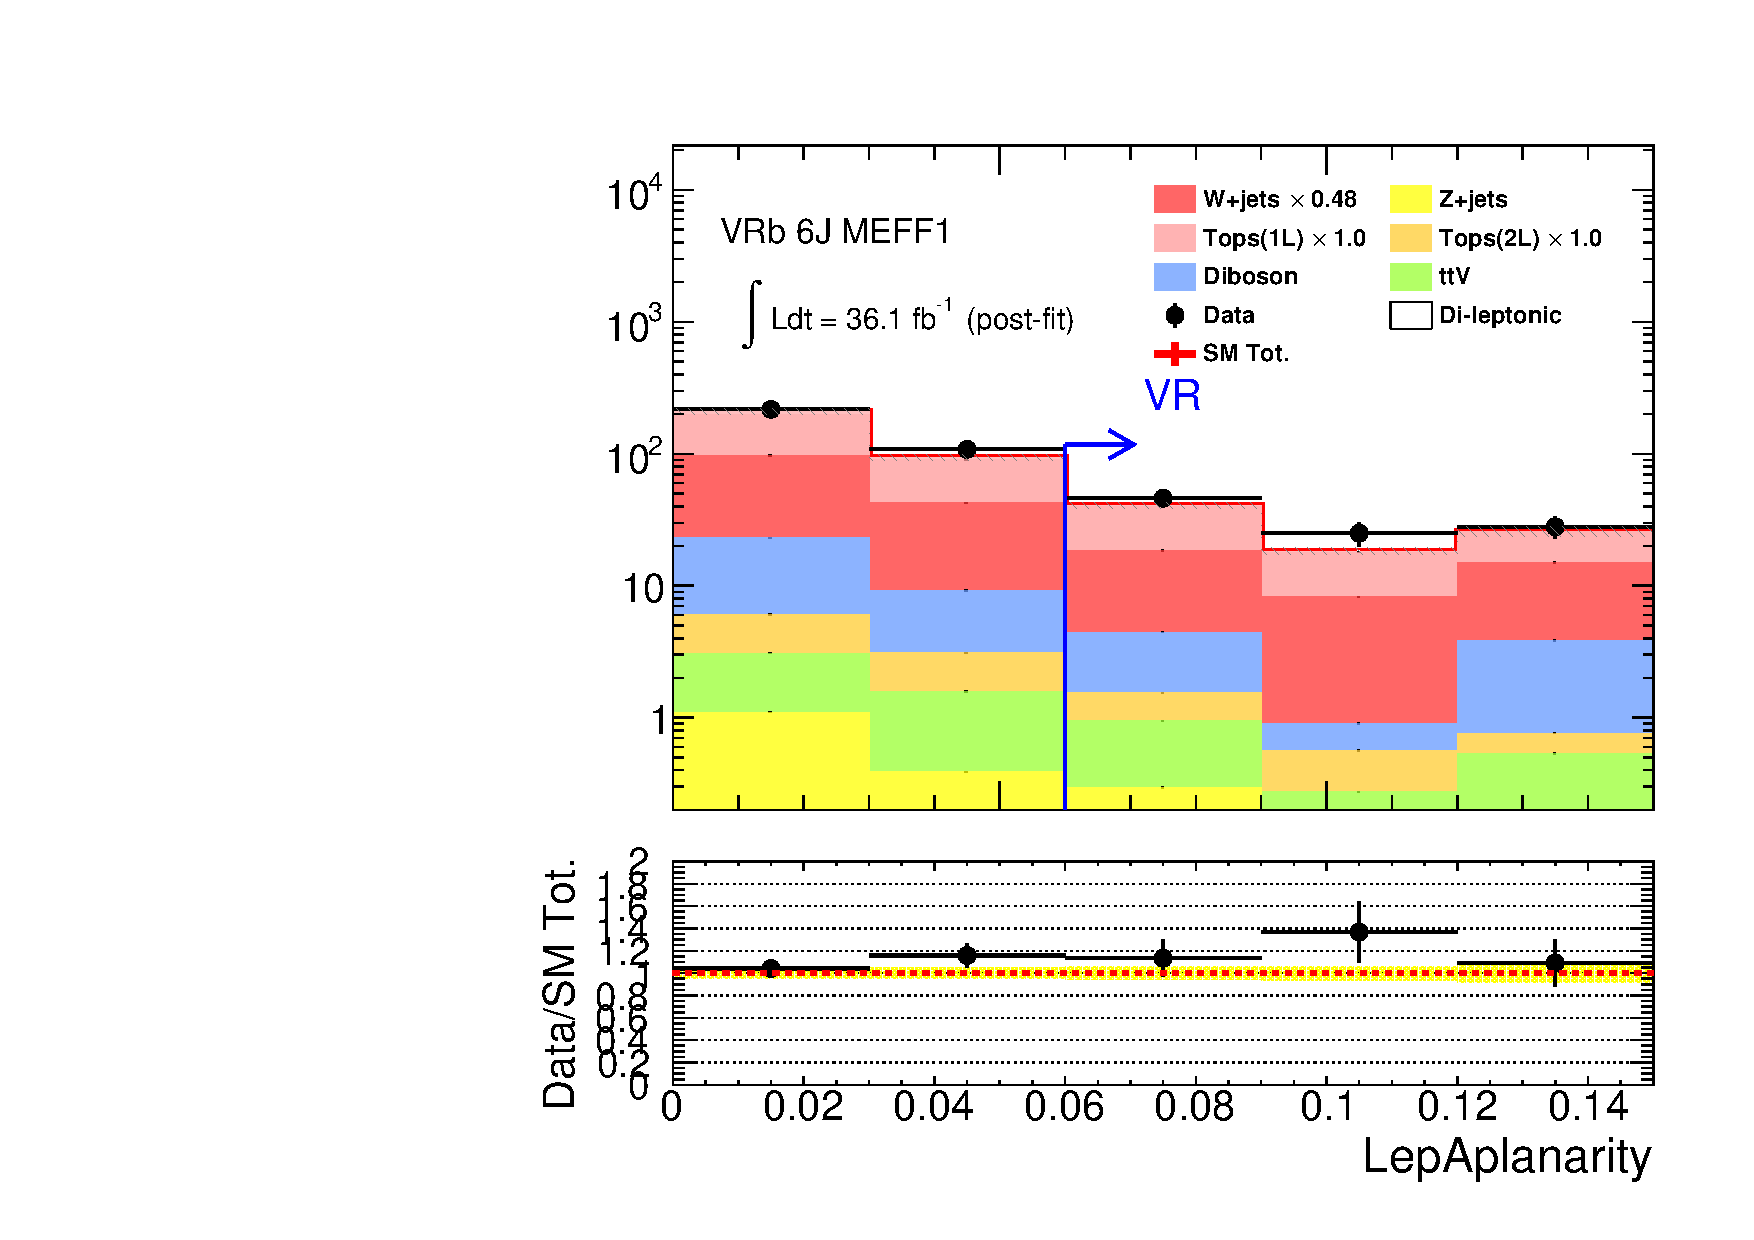
\includegraphics[width=0.41\textwidth]{figures/BGestimation/SRVRpostFit/LepAplanarity__VRb6JMEFF1_no_LepAplanarity_postFit_2SFconfig_noYields_objRep.pdf}}
    \subfigure[]{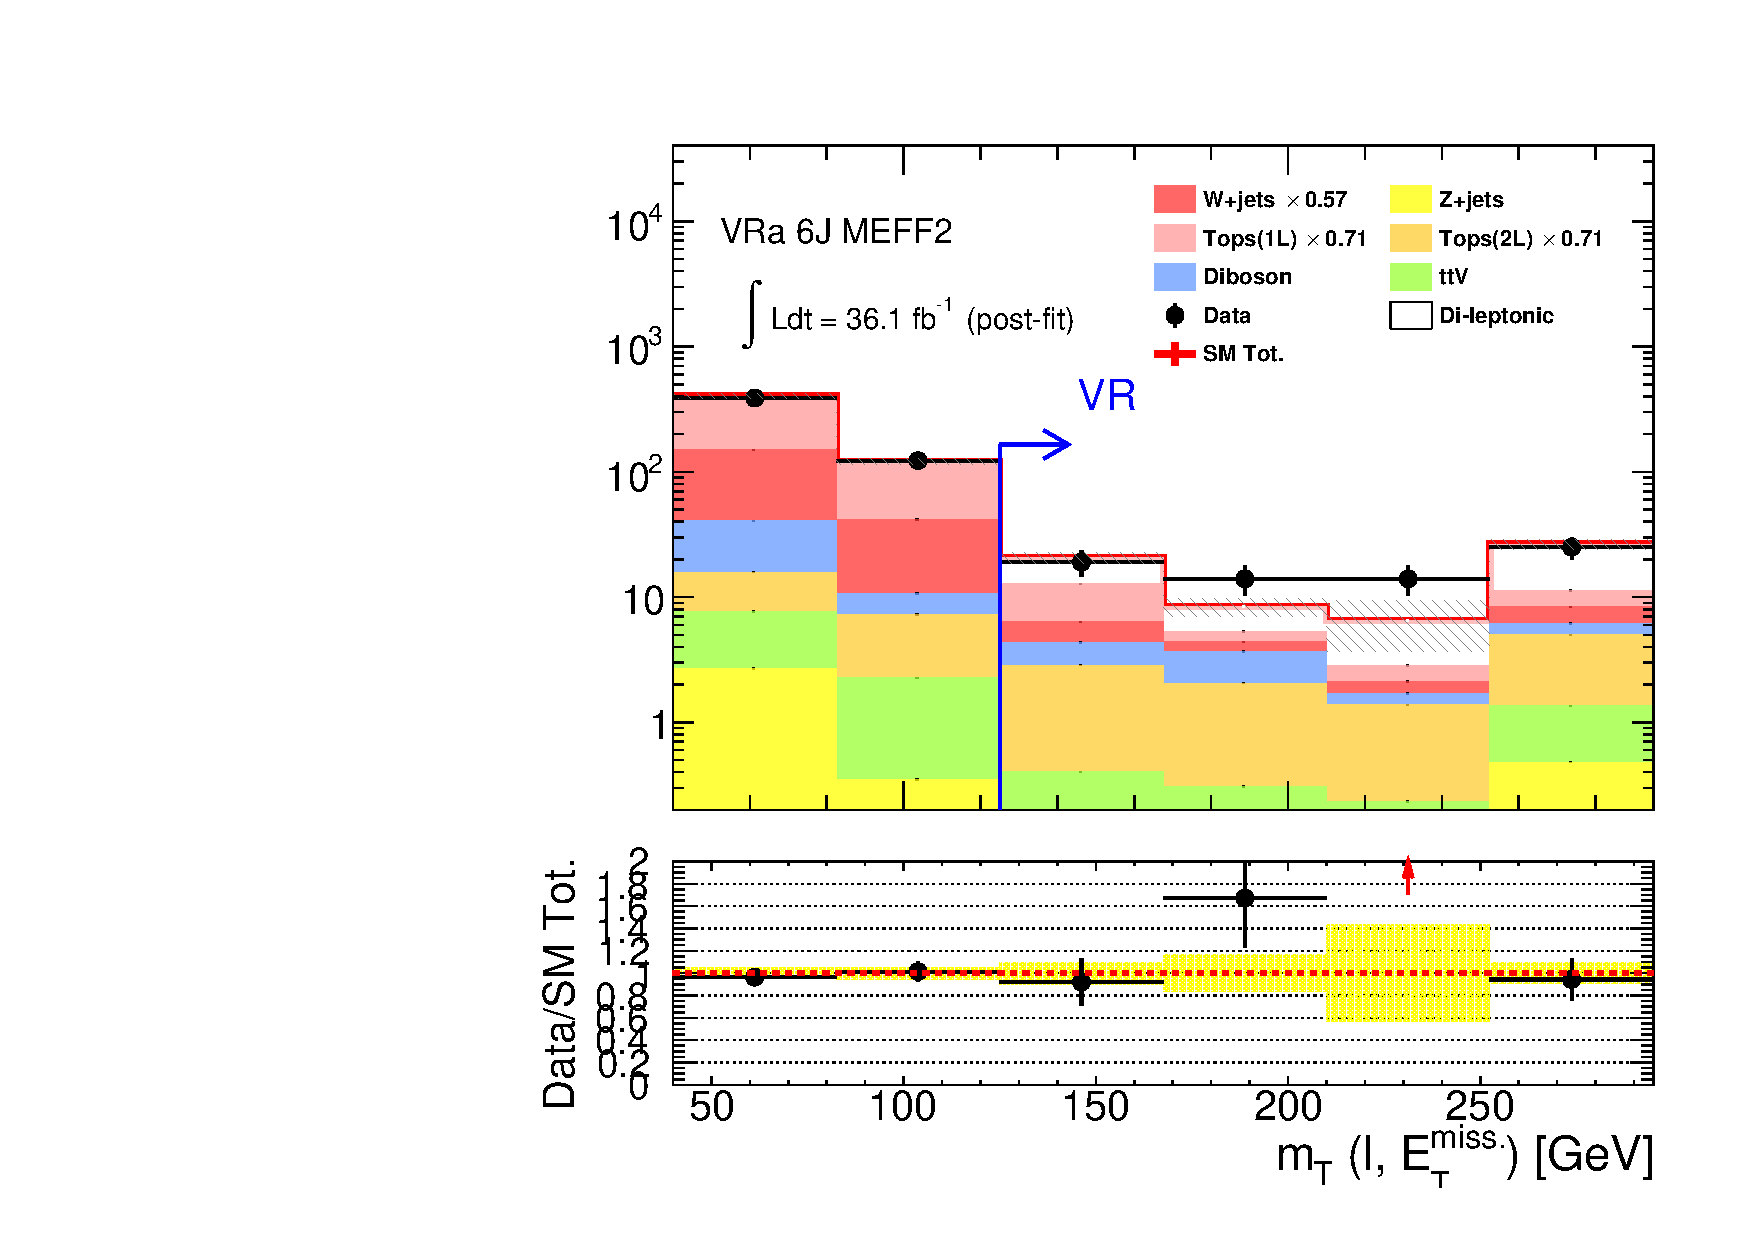
\includegraphics[width=0.41\textwidth]{figures/BGestimation/SRVRpostFit/mt__VRa6JMEFF2_no_mt_postFit_2SFconfig_noYields_objRep.pdf}}
    \subfigure[]{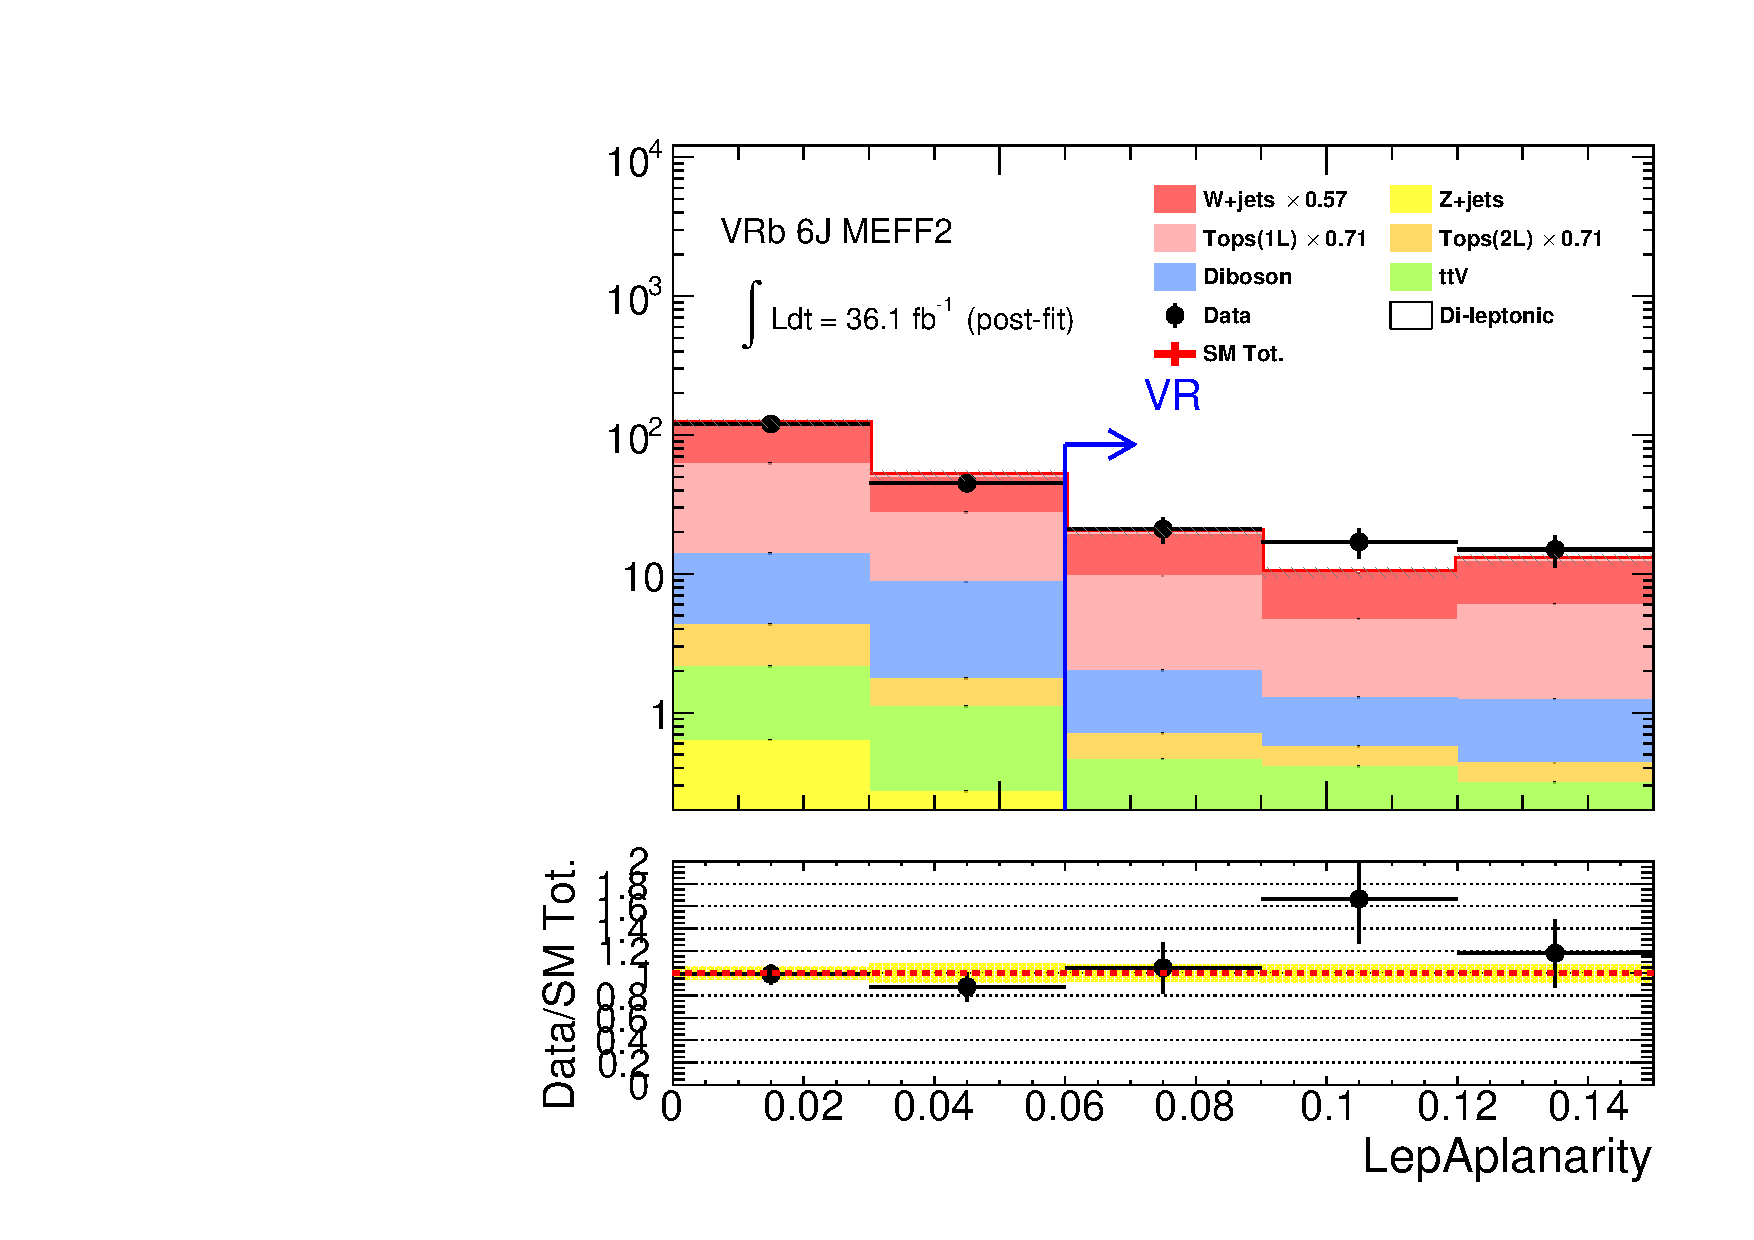
\includegraphics[width=0.41\textwidth]{figures/BGestimation/SRVRpostFit/LepAplanarity__VRb6JMEFF2_no_LepAplanarity_postFit_2SFconfig_noYields_objRep.pdf}}
    \subfigure[]{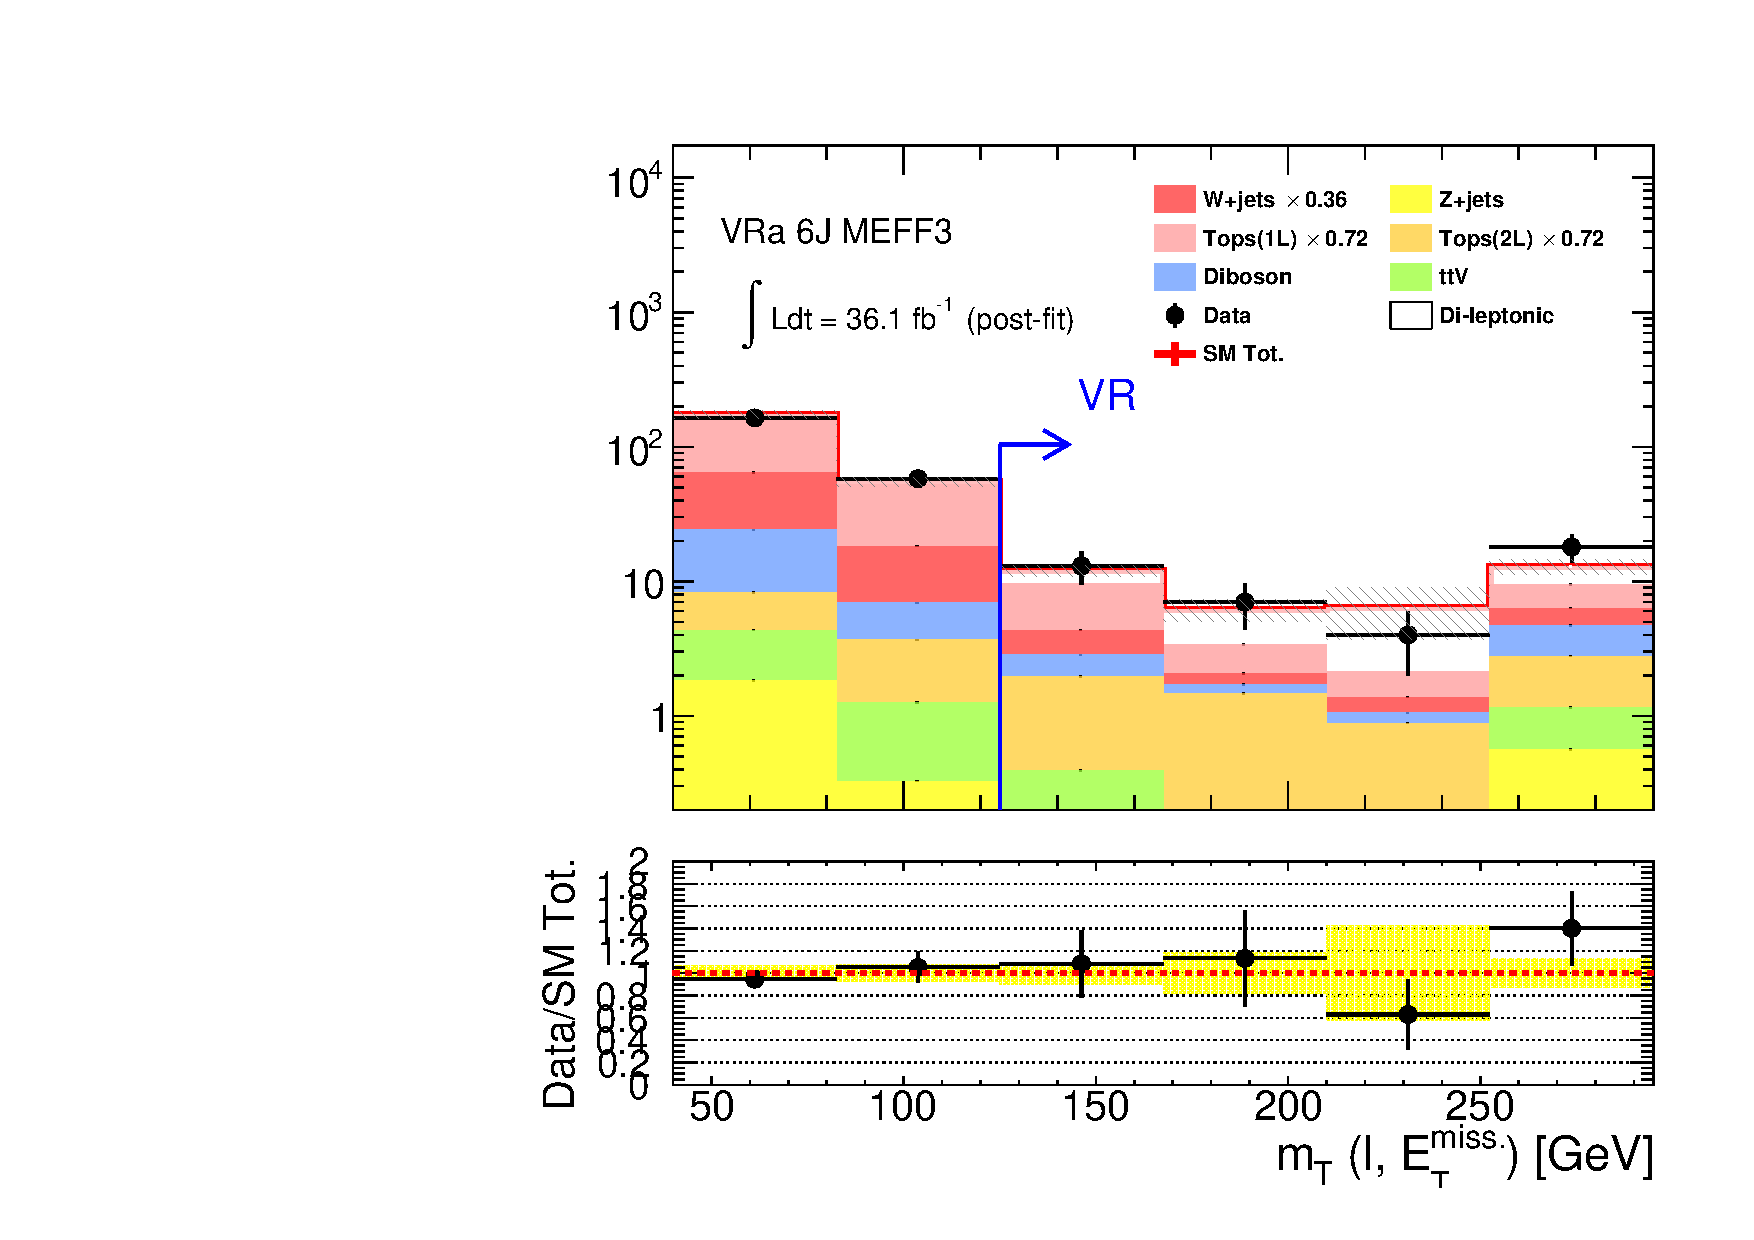
\includegraphics[width=0.41\textwidth]{figures/BGestimation/SRVRpostFit/mt__VRa6JMEFF3_no_mt_postFit_2SFconfig_noYields_objRep.pdf}}
    \subfigure[]{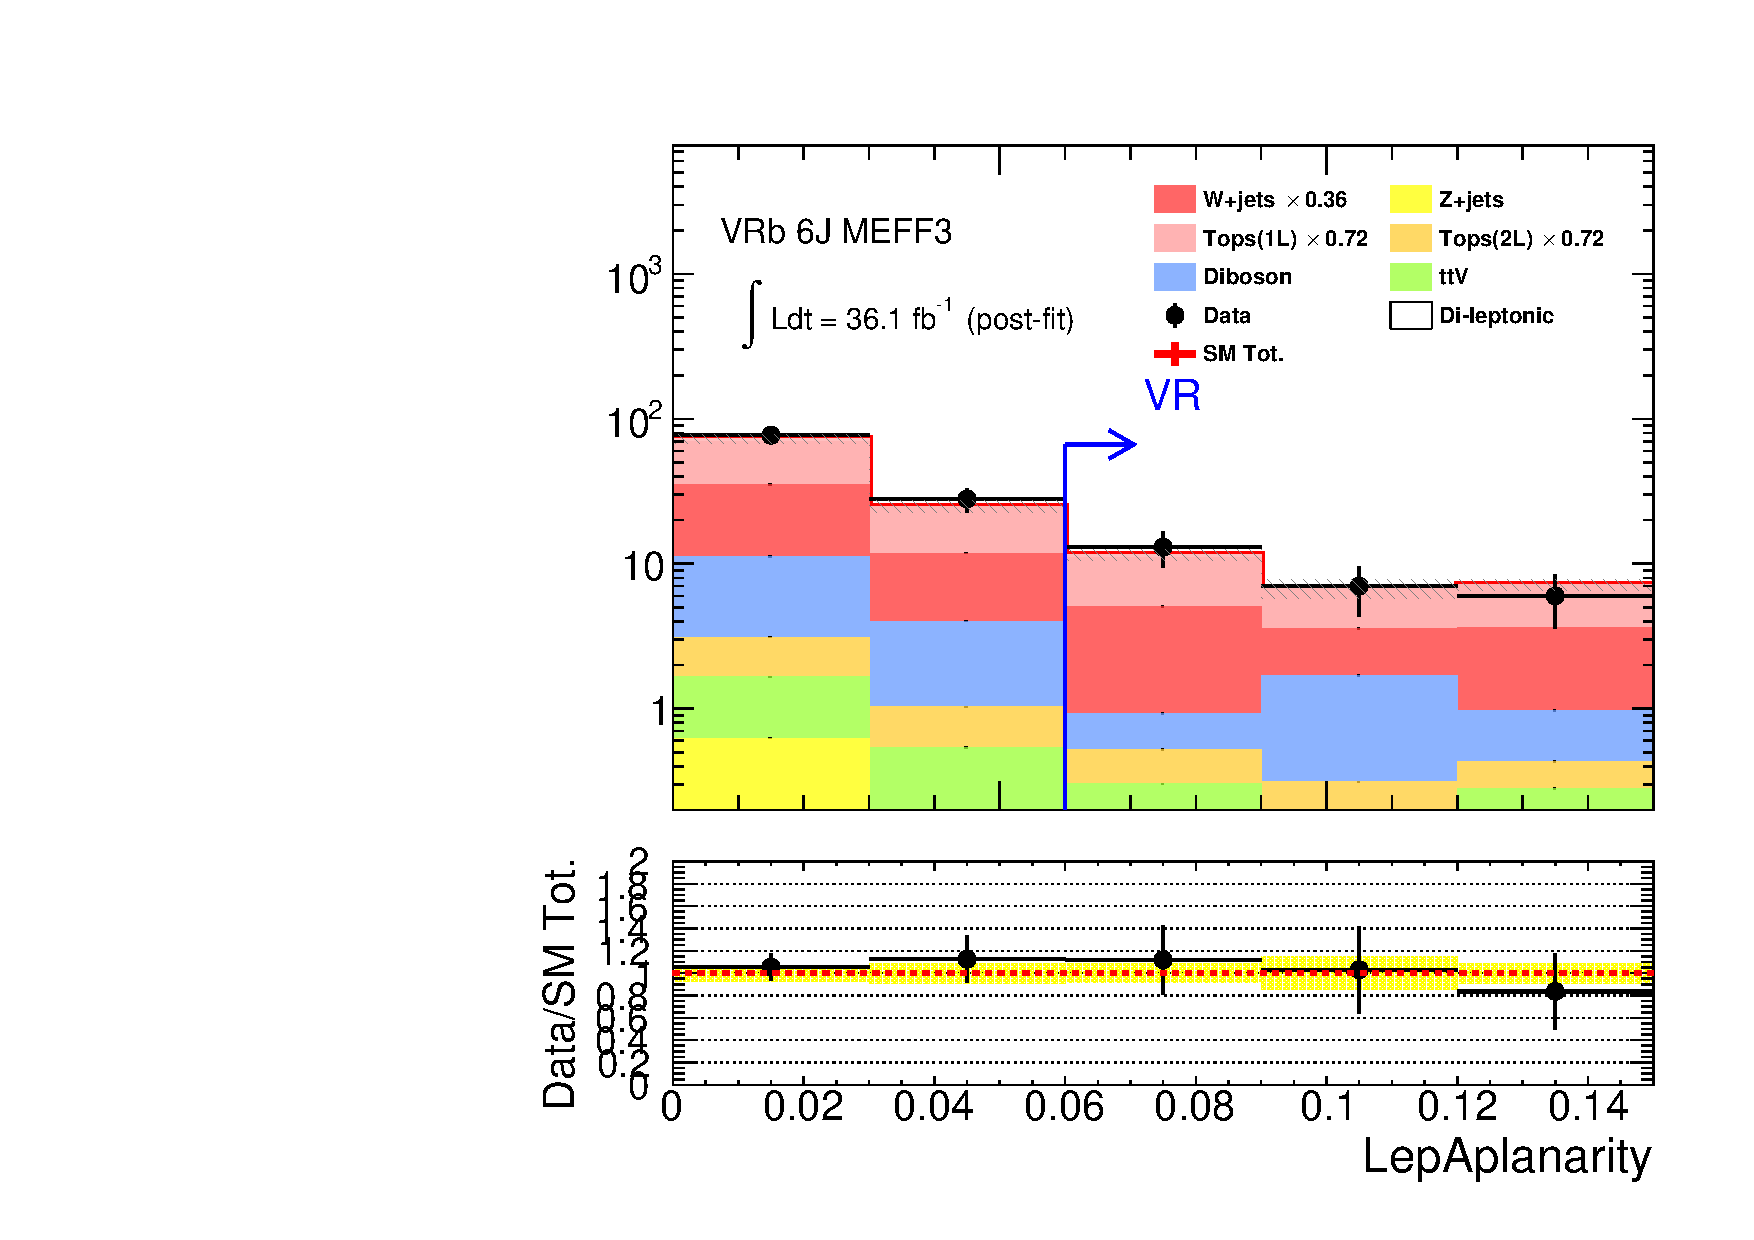
\includegraphics[width=0.41\textwidth]{figures/BGestimation/SRVRpostFit/LepAplanarity__VRb6JMEFF3_no_LepAplanarity_postFit_2SFconfig_noYields_objRep.pdf}}
    \caption{
      Post-fit distruibution of (left) $\mt$ in VRa, and (right) $\apl$ in VRb.
      (a,b) VR 6J-$\meffIncFirst$.
      (c,d) VR 6J-$\meffIncSecond$.
      (e,f) VR 6J-$\meffIncThird$.
      The yellow band in the bottom panel represents only statistical error. The overflow is included in the highest bin.  
      \label{fig::BGestimation::SRVRpostFit::VR6J}
    }
\end{figure}
%----------------------------------


\clearpage
% -------------- varx ---------
\begin{figure}[h]
  \centering
    \subfigure[]{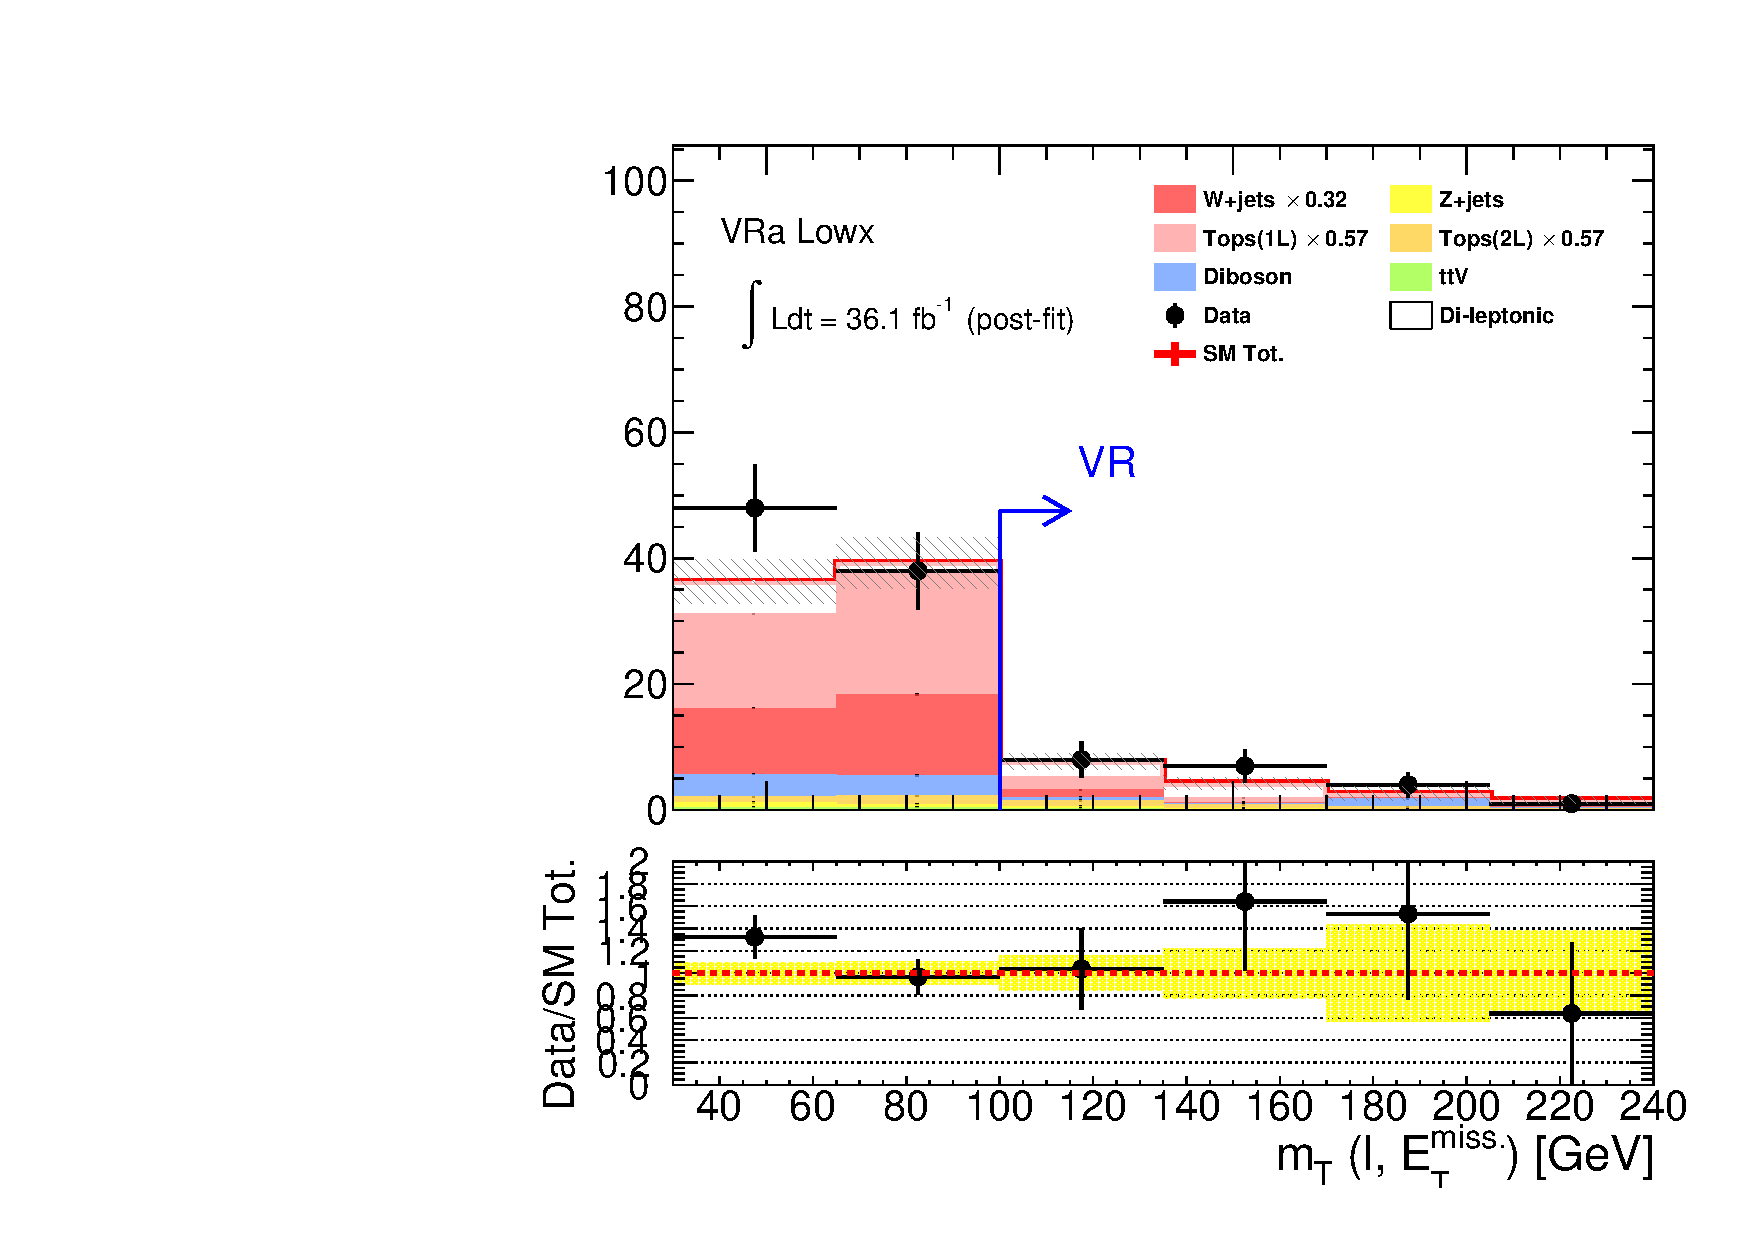
\includegraphics[width=0.41\textwidth]{figures/BGestimation/SRVRpostFit/mt__VRaLowx_no_mt_postFit_2SFconfig_noYields_objRep.pdf}}
    \subfigure[]{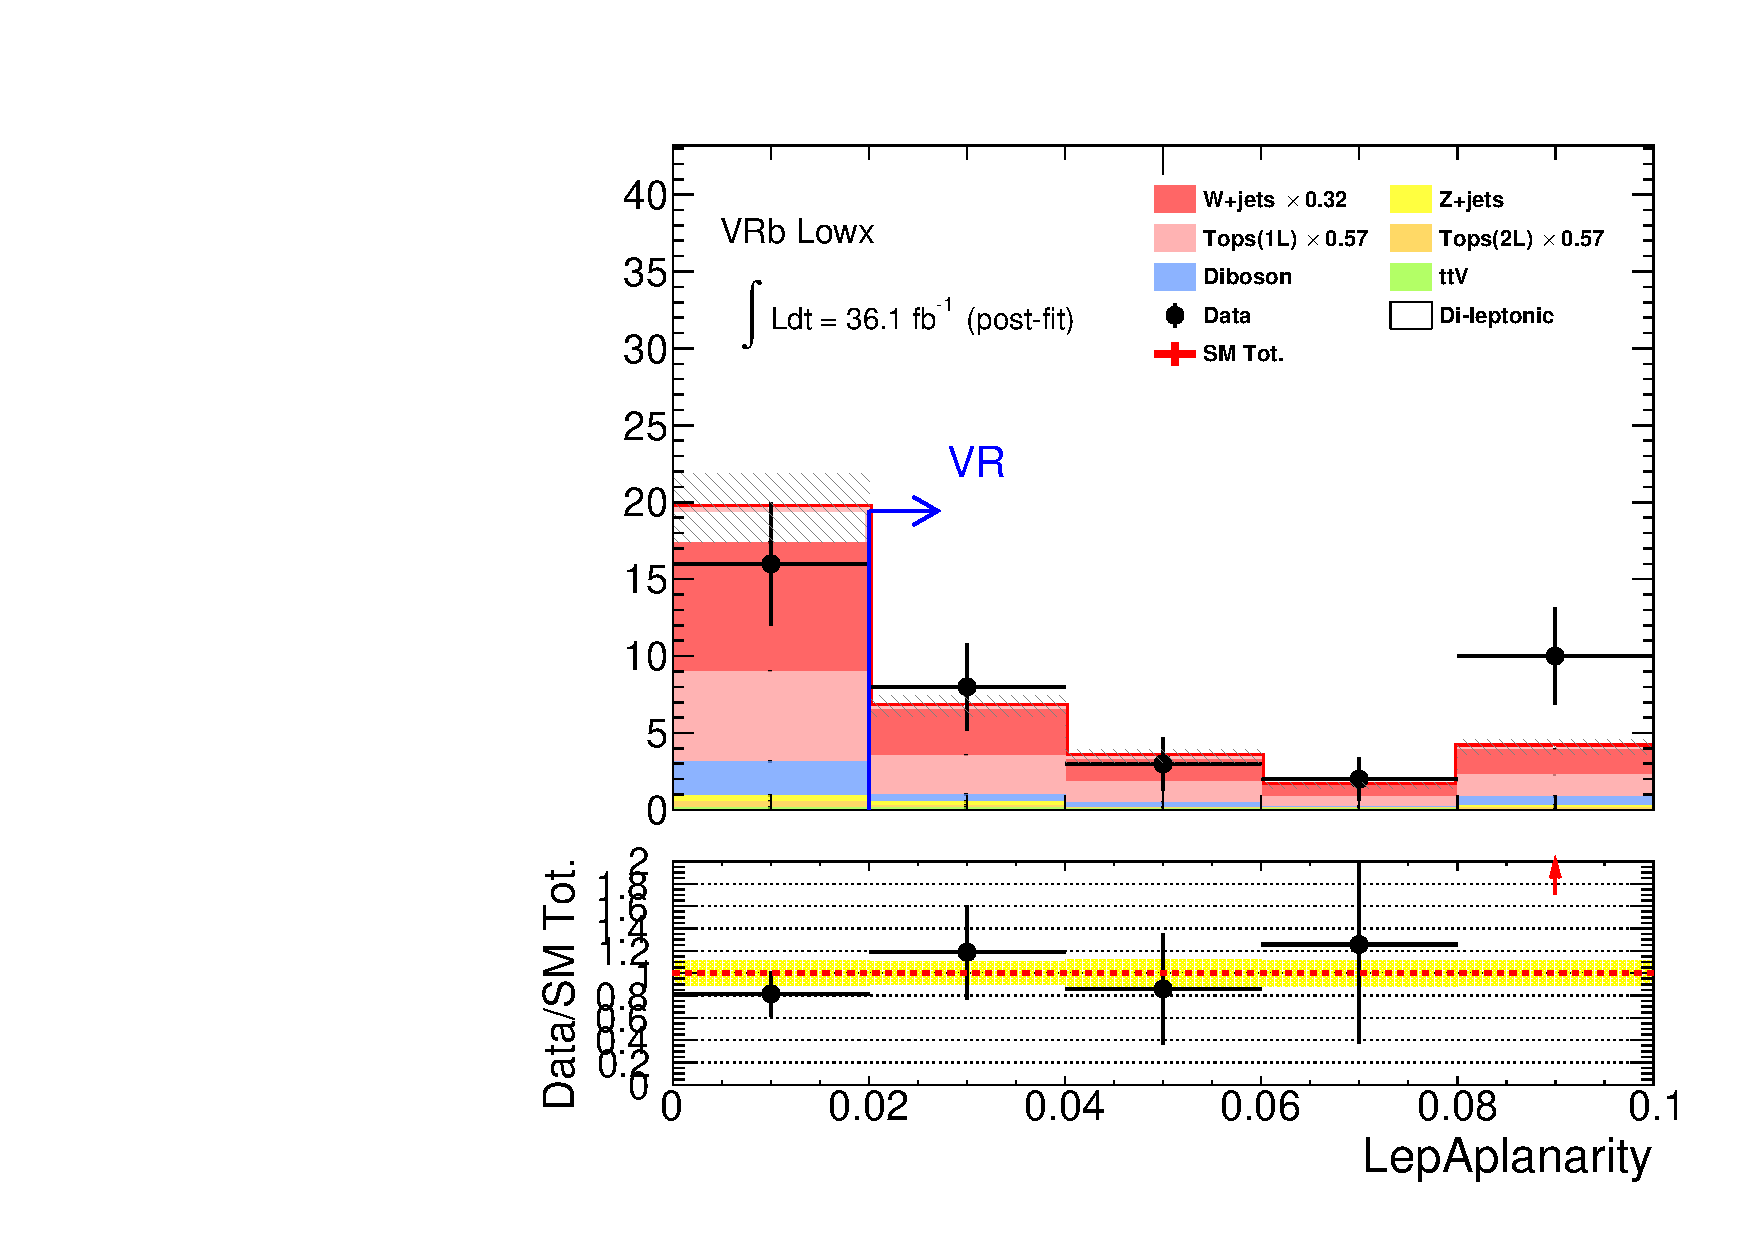
\includegraphics[width=0.41\textwidth]{figures/BGestimation/SRVRpostFit/LepAplanarity__VRbLowx_no_LepAplanarity_postFit_2SFconfig_noYields_objRep.pdf}}
    \subfigure[]{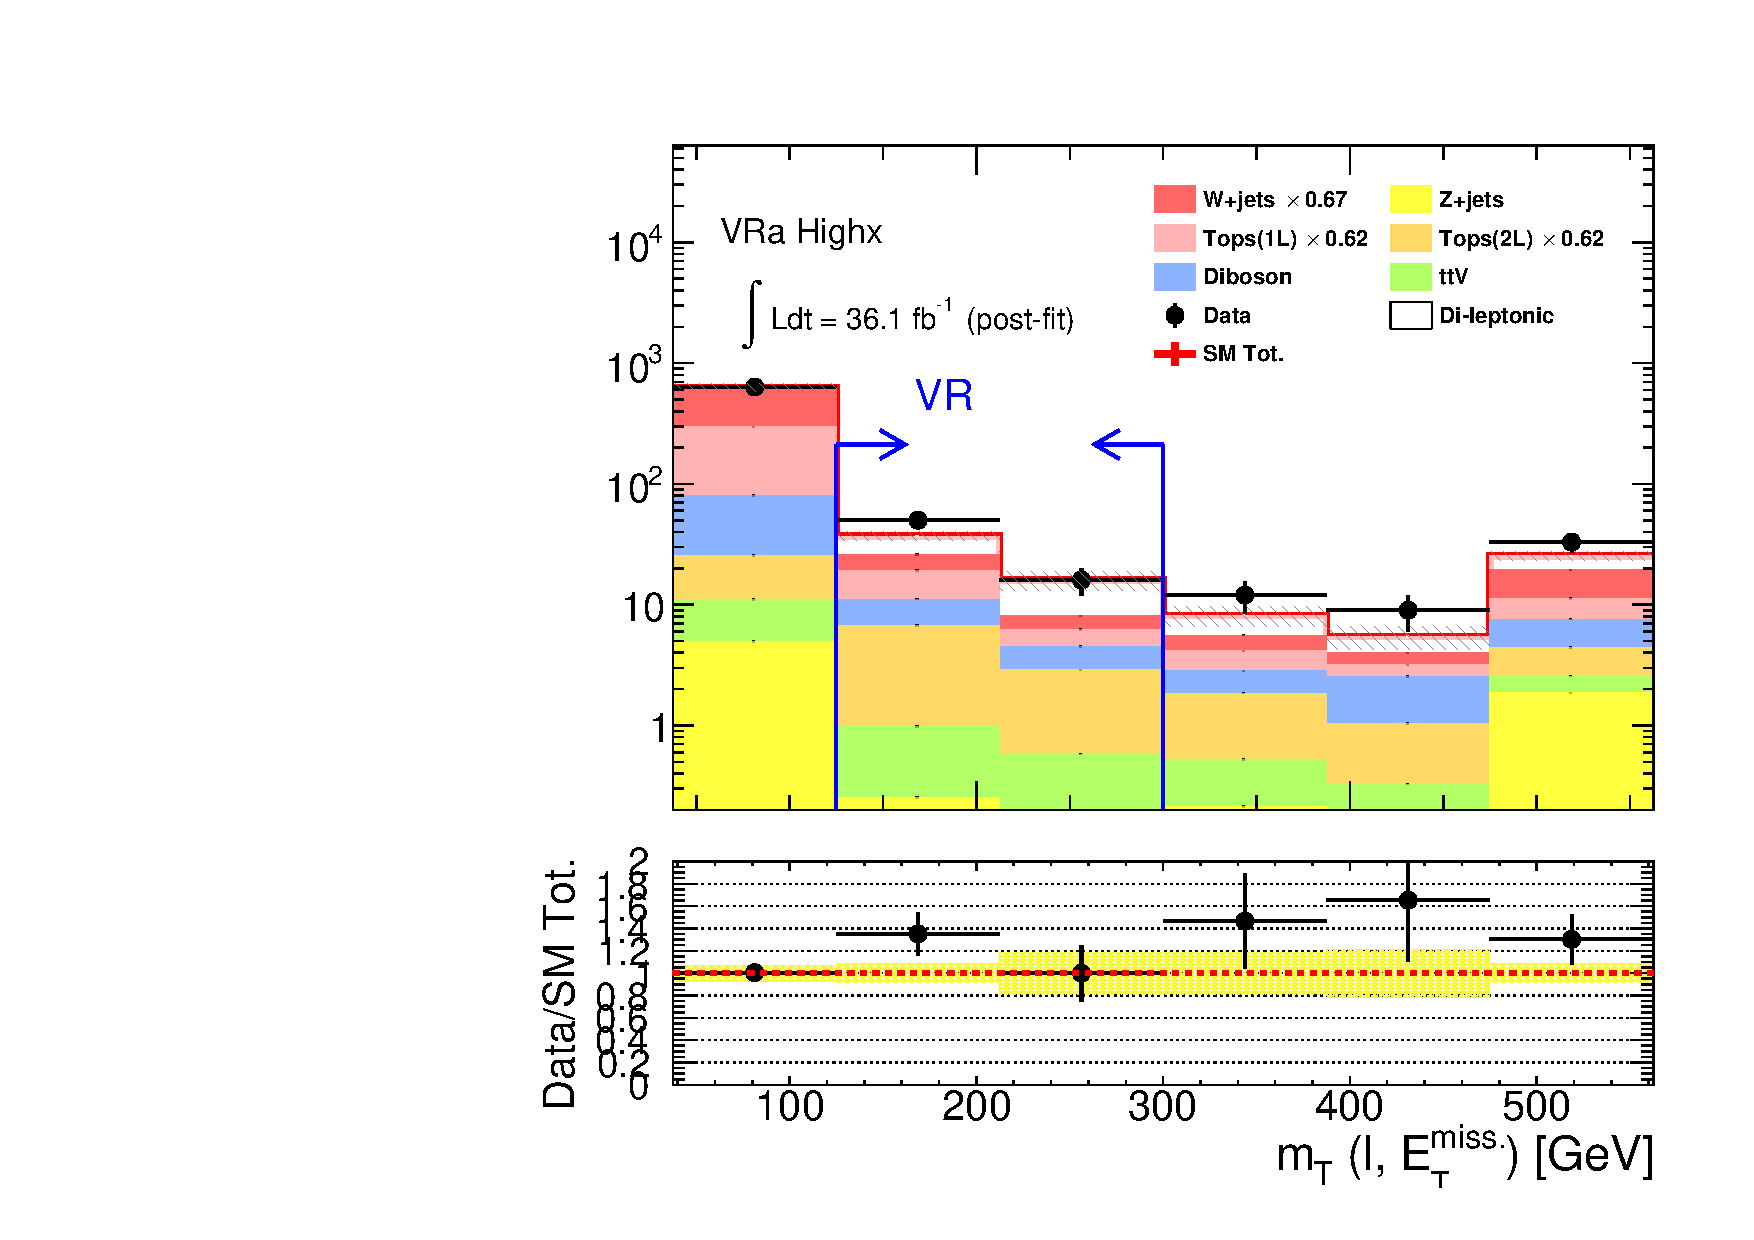
\includegraphics[width=0.41\textwidth]{figures/BGestimation/SRVRpostFit/mt__VRaHighx_no_mt_postFit_2SFconfig_noYields_objRep.pdf}}
    \subfigure[]{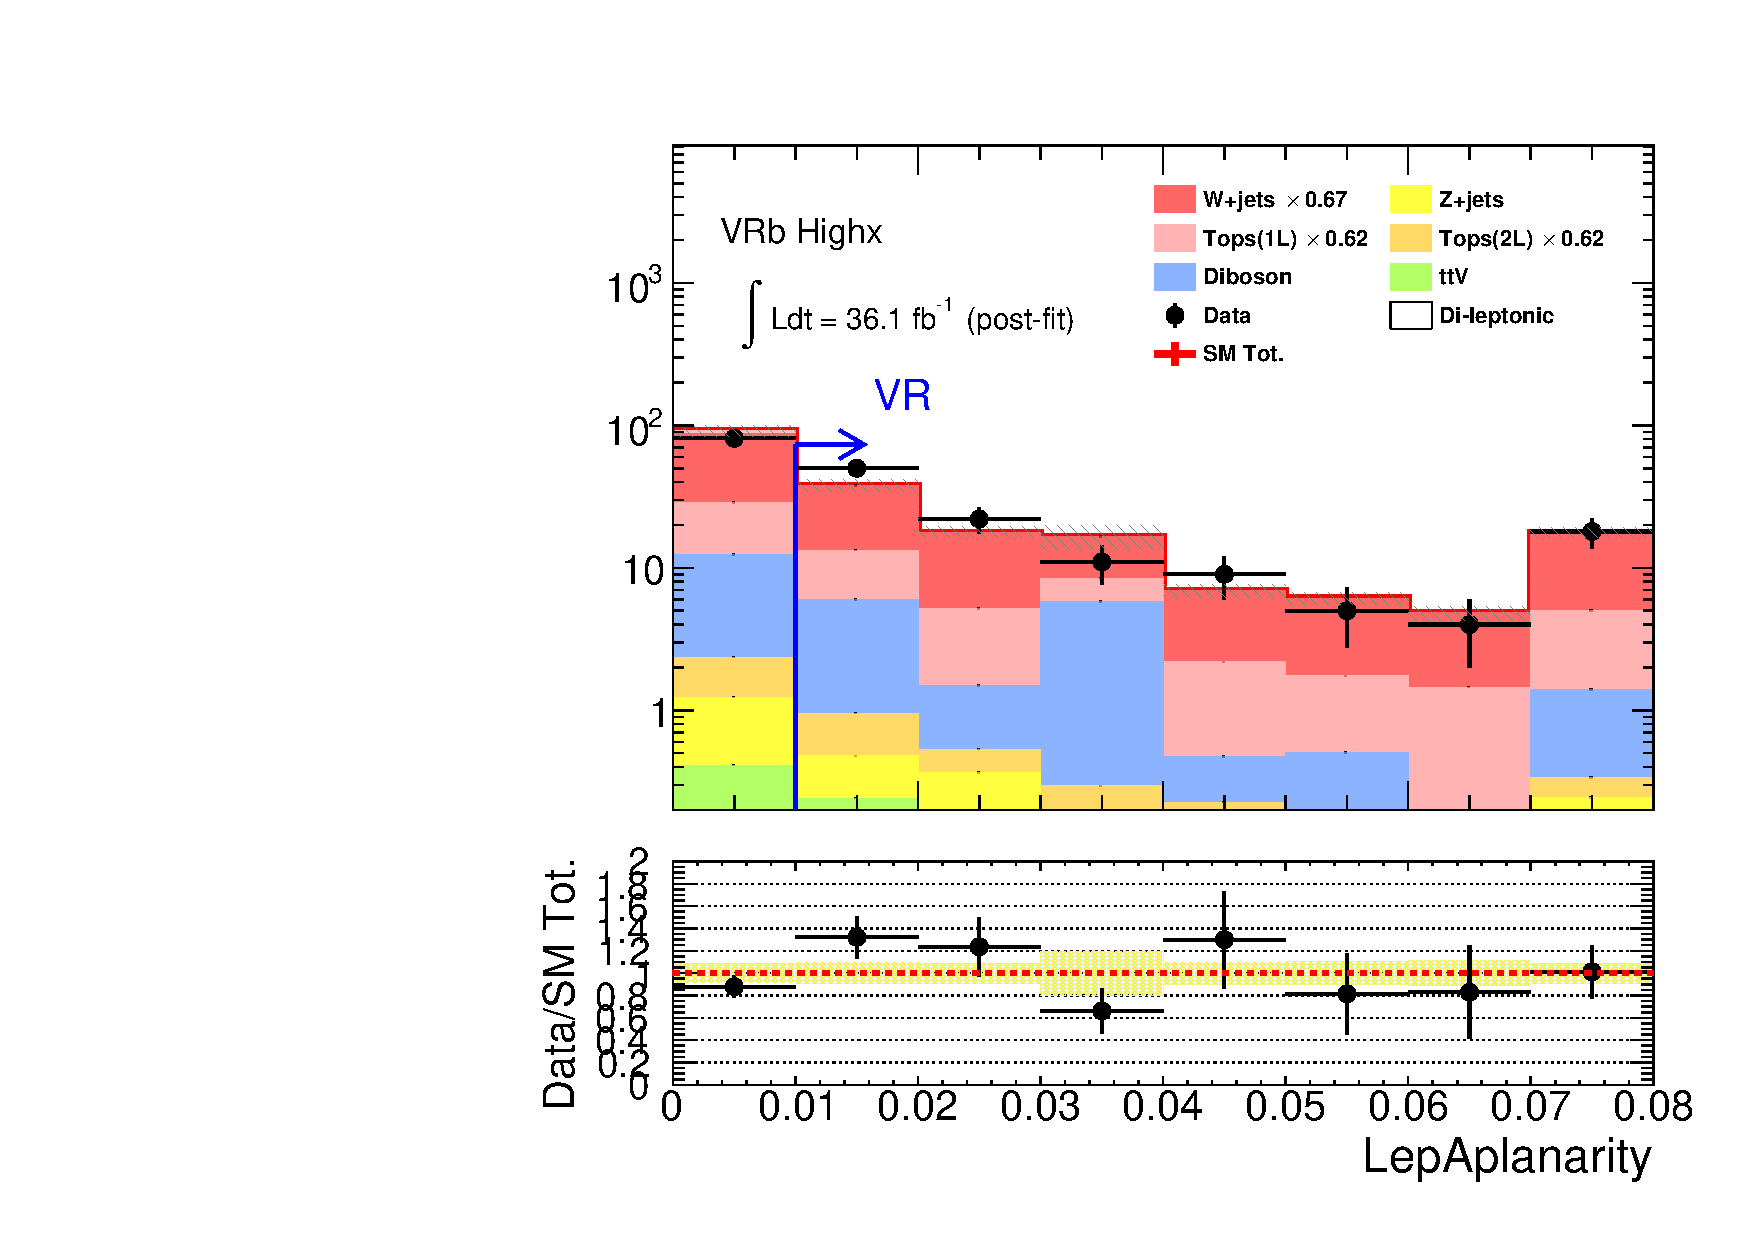
\includegraphics[width=0.41\textwidth]{figures/BGestimation/SRVRpostFit/LepAplanarity__VRbHighx_no_LepAplanarity_postFit_2SFconfig_noYields_objRep.pdf}}
   \caption{   
     Post-fit distruibution of (left) $\mt$ in VRa, and (right) $\apl$ in VRb.
     (a,b) VR Low-x.
     (c,d) VR High-x.
     The yellow band in the bottom panel represents only statistical error. The overflow is included in the highest bin.  
     \label{fig::BGestimation::SRVRpostFit::VRVarx}
   }
\end{figure}
% ----------------------------------------------

\clearpage
% -------------- 3B ---------
\begin{figure}[h]
  \centering
    \subfigure[]{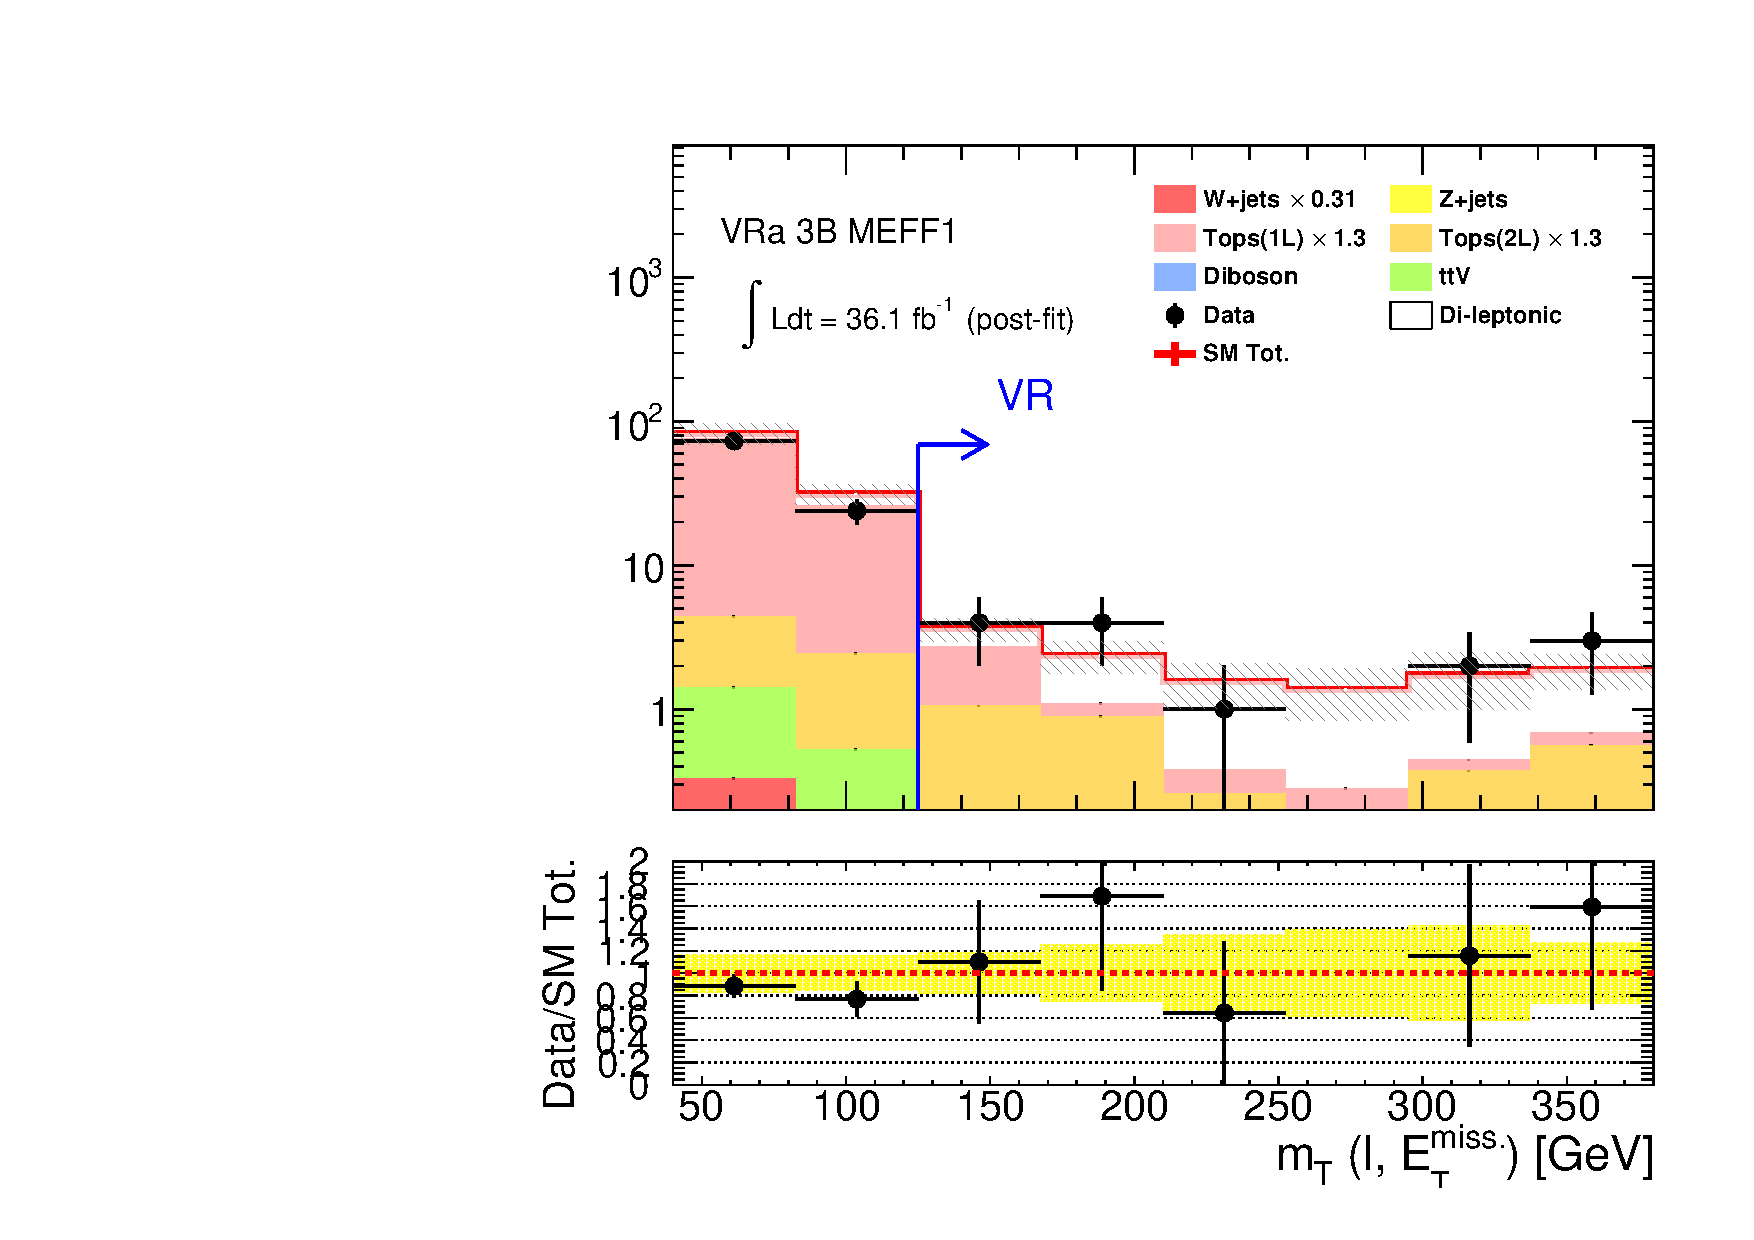
\includegraphics[width=0.41\textwidth]{figures/BGestimation/SRVRpostFit/mt__VRa3BMEFF1_no_mt_postFit_2SFconfig_noYields_objRep.pdf}}
    \subfigure[]{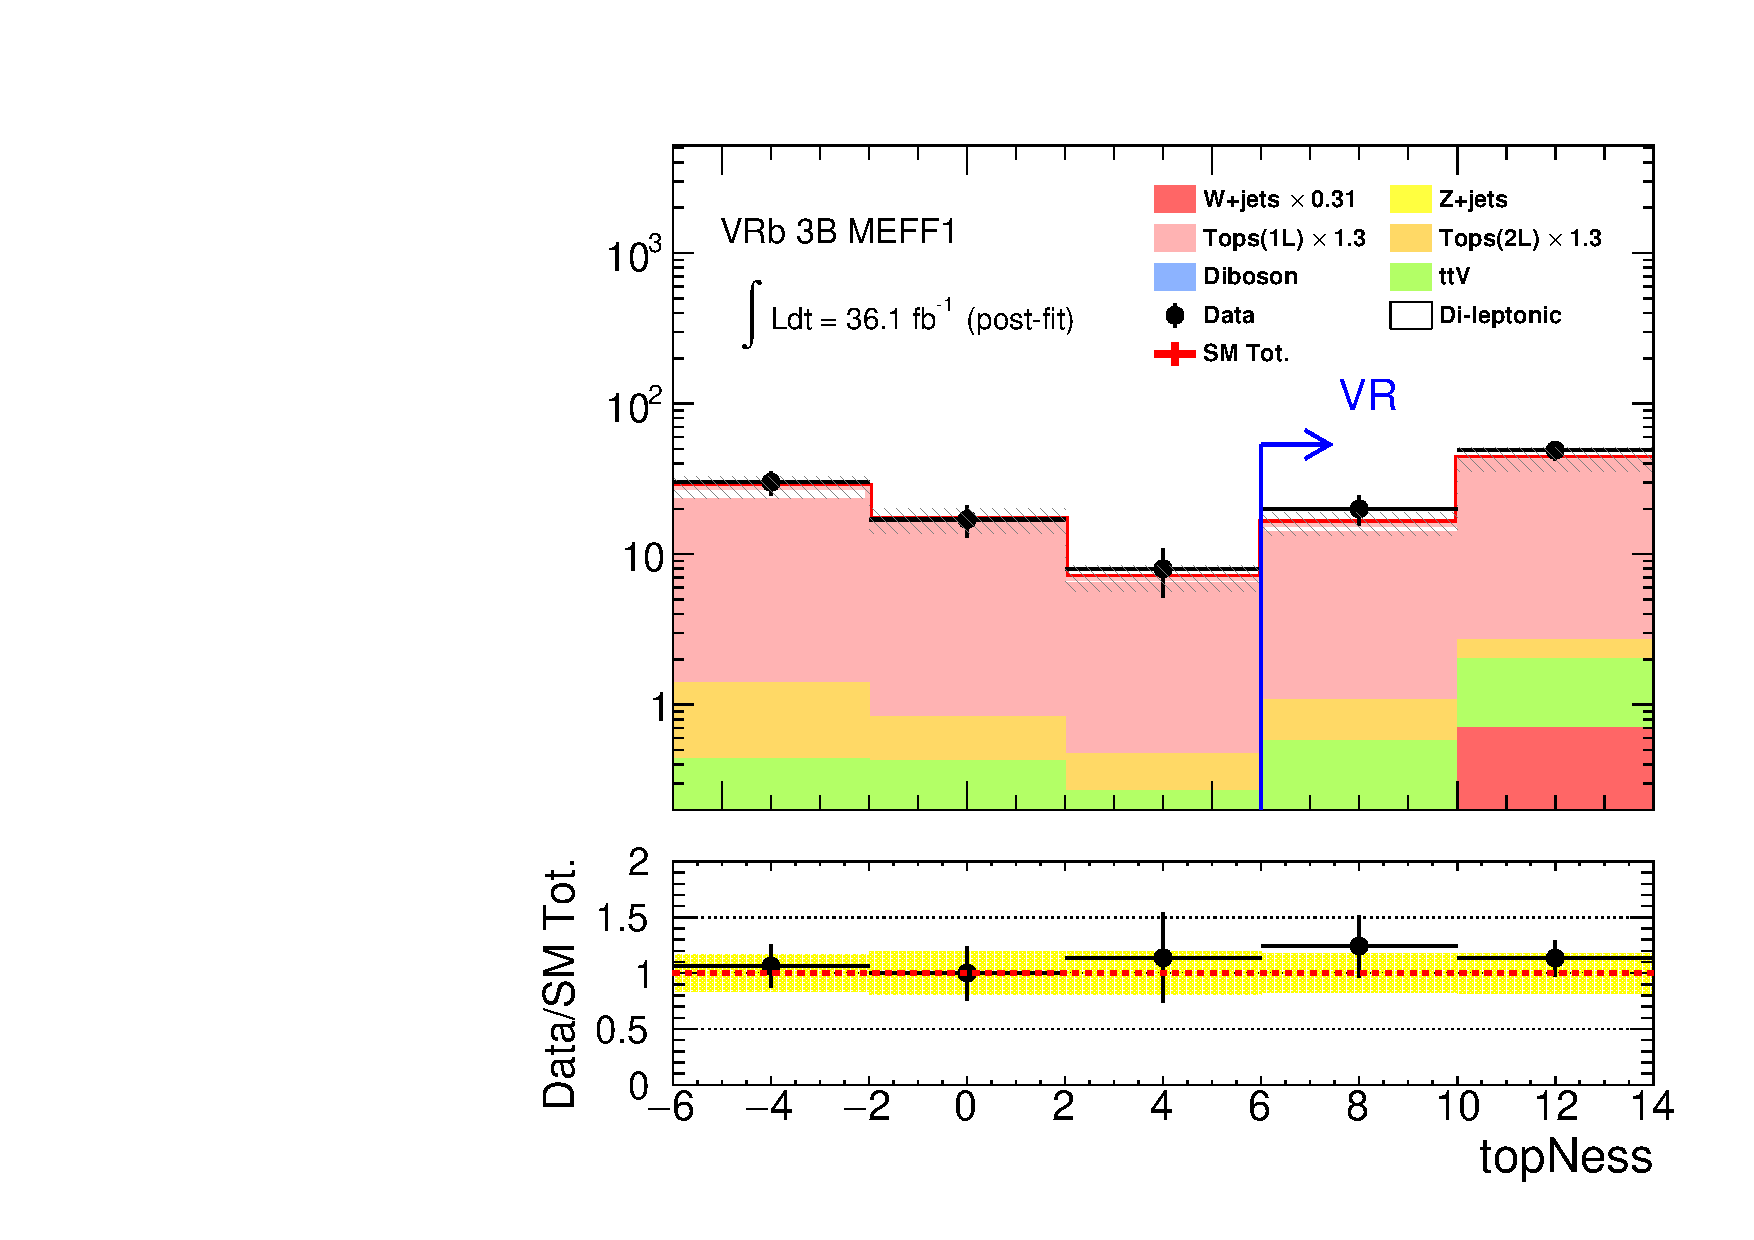
\includegraphics[width=0.41\textwidth]{figures/BGestimation/SRVRpostFit/topNess__VRb3BMEFF1_no_topNess_postFit_2SFconfig_noYields_objRep.pdf}}
    \subfigure[]{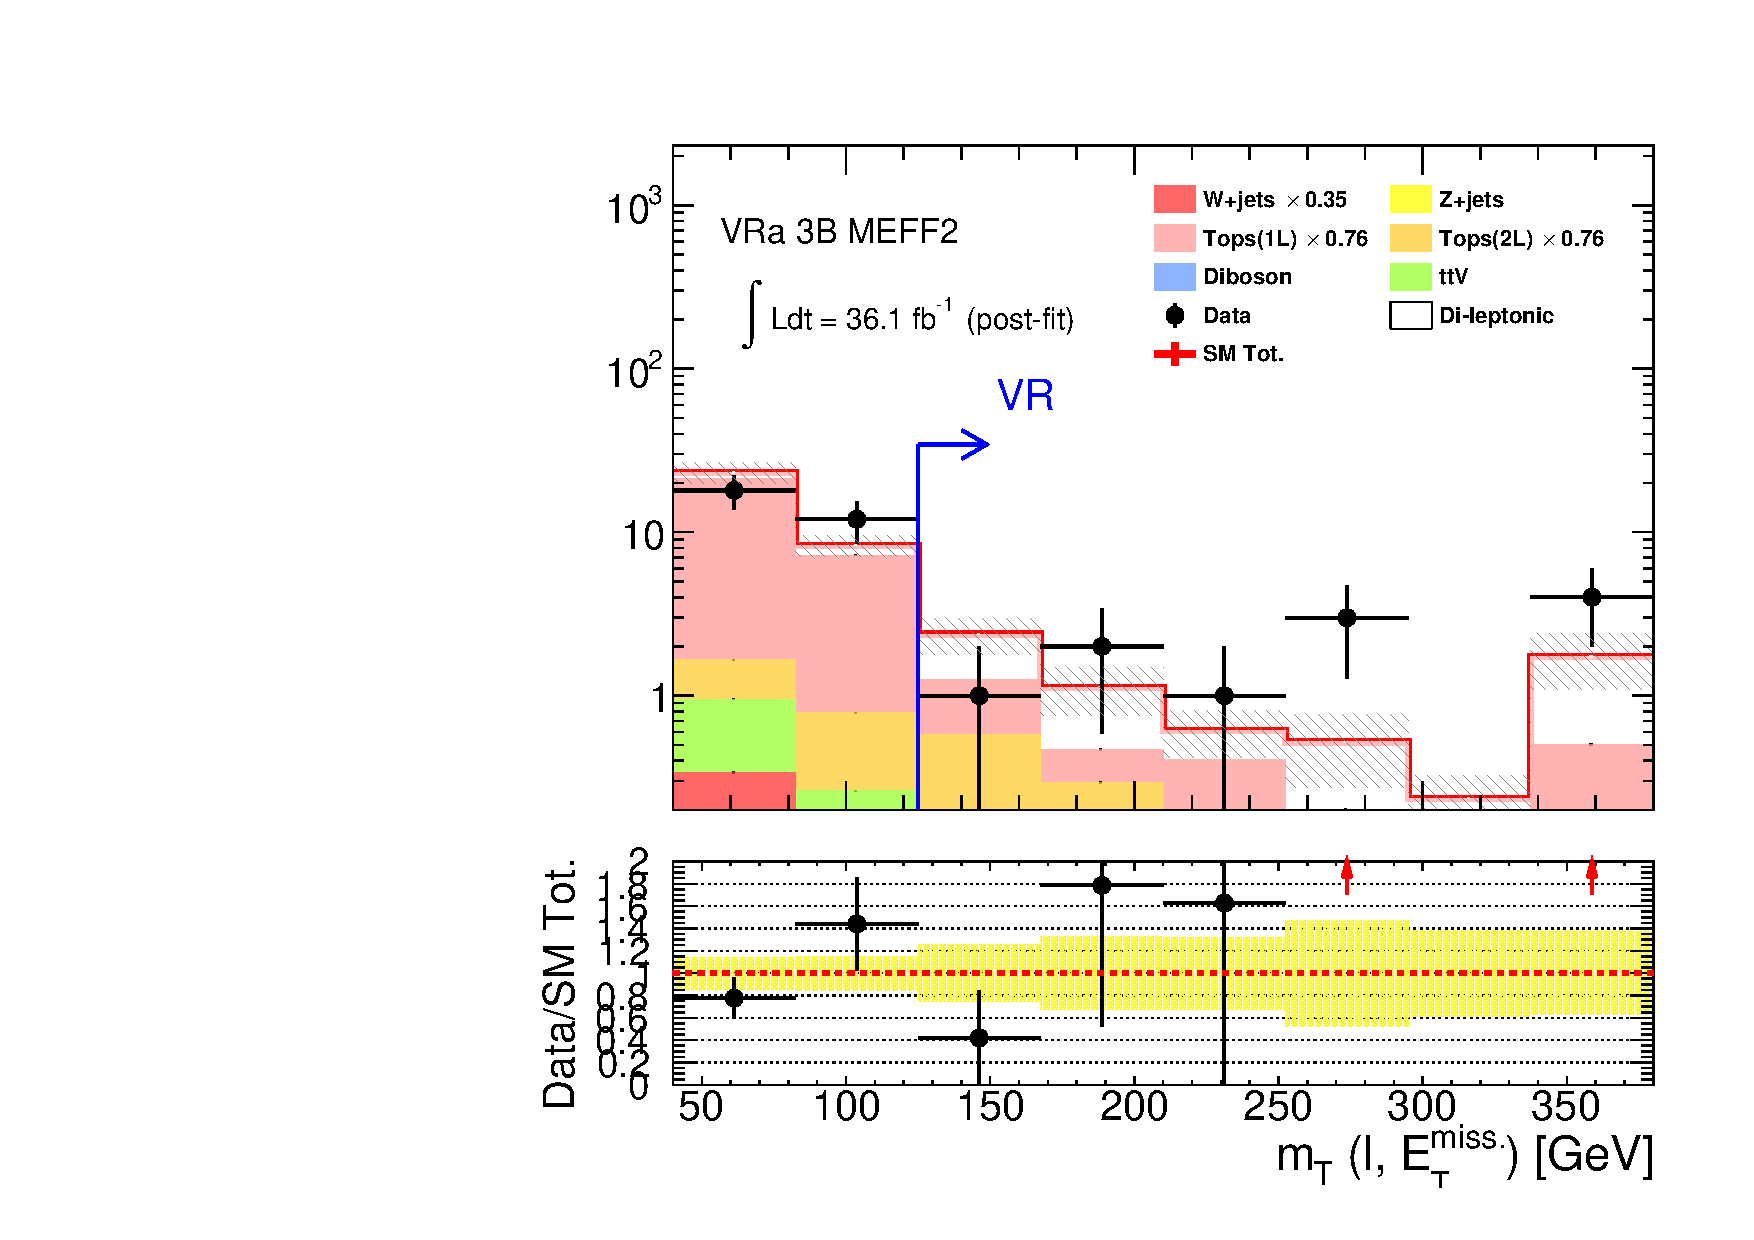
\includegraphics[width=0.41\textwidth]{figures/BGestimation/SRVRpostFit/mt__VRa3BMEFF2_no_mt_postFit_2SFconfig_noYields_objRep.pdf}}
    \subfigure[]{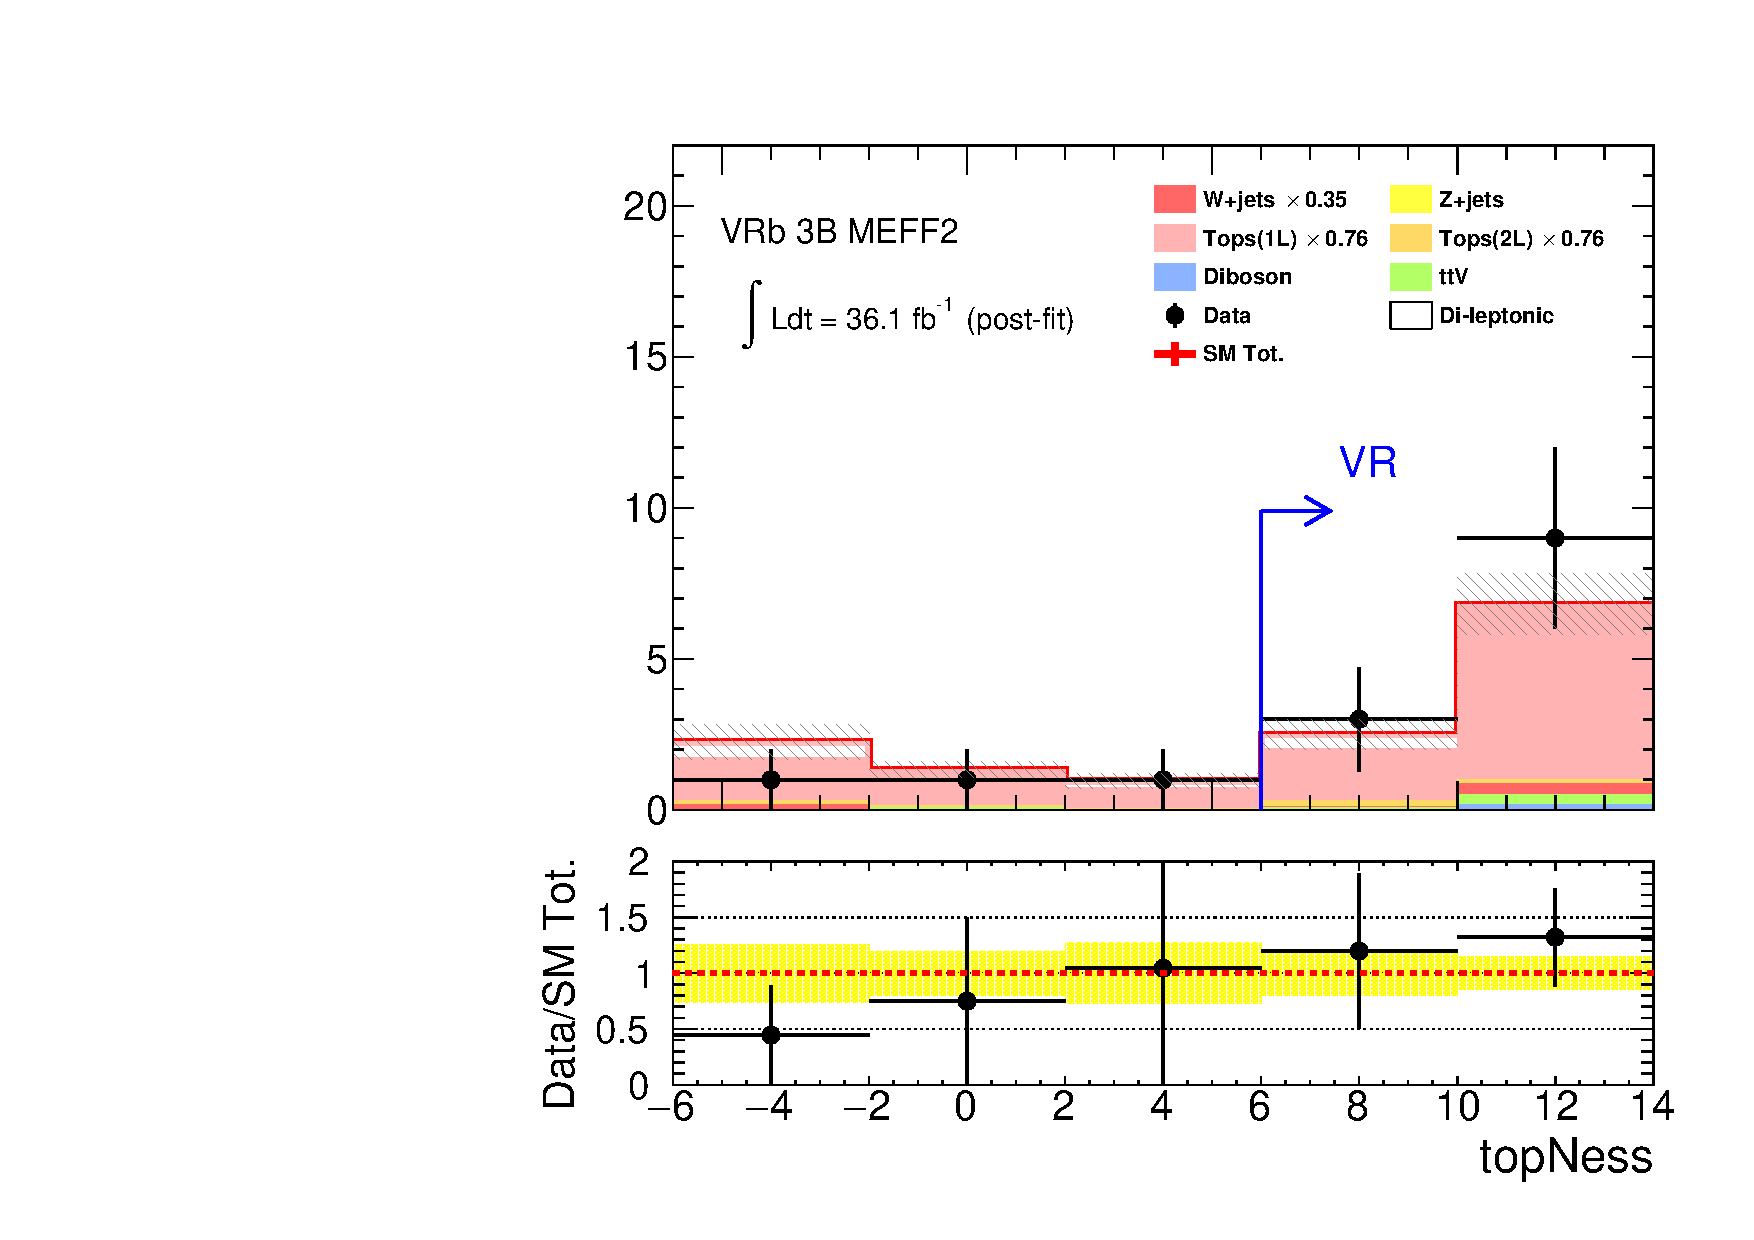
\includegraphics[width=0.41\textwidth]{figures/BGestimation/SRVRpostFit/topNess__VRb3BMEFF2_no_topNess_postFit_2SFconfig_noYields_objRep.pdf}}
    \caption{   
      Post-fit distruibution of (left) $\mt$ in VRa, and (right) topness in VRb.
      (a,b) VR 3B-$\meffIncFirst$.
      (c,d) VR 3B-$\meffIncSecond$.
      The yellow band in the bottom panel represents only statistical error. The overflow is included in the highest bin.  
      \label{fig::BGestimation::SRVRpostFit::VR3B}
    }
\end{figure}
